\documentclass{mynotes}

\usepackage{amsmath,amsfonts,amsthm,amssymb}
\usepackage{bm}
%\usepackage{indentfirst}
\usepackage{algorithm}
\usepackage{algpseudocode}
\usepackage{emoji}

\usepackage{subcaption}
\usepackage{multicol}
\usepackage{multirow}

\usepackage{tikz}
\usepackage{listings}

\usepackage{epigraph}

\usepackage{import}
\usepackage{nomencl}
\renewcommand{\nomname}{Ký hiệu chung}
\makenomenclature

\usepackage{tabularx}

\usepackage{blindtext}
\usepackage{minitoc}
\usepackage{wrapfig}
\setlength{\columnsep}{0.5cm}

%\usepackage{txfonts}


\renewcommand*{\epigraphsize}{\normalsize}
\PassOptionsToPackage{hyphens}{url}

\newcommand{\MC}{\mathcal{C}}
\newcommand{\FF}{\mathbb{F}}
\newcommand{\NN}{\mathbb{N}}
\newcommand{\ZZ}{\mathbb{Z}}
\newcommand{\QQ}{\mathbb{Q}}
\newcommand{\RR}{\mathbb{R}}
\newcommand{\II}{\mathbb{I}}
\newcommand{\CC}{\mathbb{C}}

% affine space
\newcommand{\Vv}{\mathcal{V}}
\newcommand{\Aa}{\mathcal{A}}

\DeclareMathOperator{\Ima}{im}
\DeclareMathOperator{\tr}{tr}
\DeclareMathOperator{\rank}{rank}
\DeclareMathOperator{\sign}{sign}
\DeclareMathOperator{\spa}{spa}
\DeclareMathOperator{\sgn}{sgn}
\DeclareMathOperator{\lb}{label}
\DeclareMathOperator{\wt}{wt}
\DeclareMathOperator{\Aut}{Aut}
\DeclareMathOperator{\lcm}{lcm}

\setlength{\parskip}{4pt}
\setlength{\extrarowheight}{4pt}

\addbibresource{references.bib}

\setcounter{tocdepth}{1}
\setcounter{parttocdepth}{3}

\renewcommand{\ptctitle}{Phần~\thepart: Nội dung}
\renewcommand{\ptifont}{\Large\bf}
\renewcommand{\ptcfont}{\normalsize\rm}

\setlist[itemize,enumerate]{noitemsep,nosep,leftmargin=*}

% Problem
\pgfdeclarehorizontalshading{problembackground}{100bp}
    {color(0bp)=(gray!40); color(100bp)=(black!5)}
\pgfdeclarehorizontalshading{problemtitle}{100bp}
    {color(0bp)=(violet!40); color(100bp)=(black!5)}

\newcounter{problem}[section]
\newenvironment{problem}[1][]{
    \stepcounter{problem}
    \ifstrempty{#1}
    {
        \mdfsetup{
            frametitle={
                \tikz[baseline=(current bounding box.east),outer sep=0pt]
                \node[line width=1pt,anchor=east,rectangle,rounded corners,draw=blue!20,fill=white,shading=problemtitle]
                {\strut \color{black}{Định nghĩa}~\thedefinition};
            },
        }
    }
    {
        \mdfsetup{
            frametitle={
                \tikz[baseline=(current bounding box.east),outer sep=0pt]
                \node[line width=1pt,anchor=east,rectangle,rounded corners,draw=blue!20,fill=white,shading=problemtitle]
                {#1};
            },
        }
    }
    \mdfsetup{innertopmargin=10pt,linecolor=blue!20,%
        linewidth=1pt,topline=true,%
        frametitleaboveskip=\dimexpr-\ht\strutbox\relax,
        roundcorner=10pt,
        nobreak=true,
        apptotikzsetting={%
            \tikzset{mdfbackground/.append style={shading=problembackground}}
        }
    }
    \begin{mdframed}[]\relax
}{\end{mdframed}}

\newtheorem*{solution}{Giải}

\begin{document}

\doparttoc
%\documentclass{article}

\usepackage{amsmath,amsfonts,amsthm,amssymb}
\usepackage[fontsize=14pt]{fontsize}
\usepackage{fontspec}
\usepackage{graphicx}
\usepackage{xcolor}

\setmainfont{CMU Serif}
\setsansfont{CMU Sans Serif}
%\setmonofont{FreeMono}
%%%%%%%%%%%%%%%%%%%%%%%%%%%%%%%%%%%%%%%%%%

%%%%%%%%%%%%%%%%%%%%%%%%%%%%%%%%%%%%%%%%%%
% Layout part
\usepackage{geometry}
\geometry{a4paper,top=2cm,left=2cm,bottom=2cm,right=2cm,
        headheight=110pt}

\begin{document}
\begin{titlepage}
    \begin{center}
        \begin{tabular}{c c c c c}
            {\Huge TOÁN} & & & & \\
            & {\Huge\color{red} HỌC} & & & \\
            & & \& & & \\ 
            & & & {\Huge\color{green} TUỔI} & \\
            & & & & {\Huge\color{blue} TRẺ}
        \end{tabular}
    \end{center}

    \begin{center}
        \begin{tabular}{c c}
                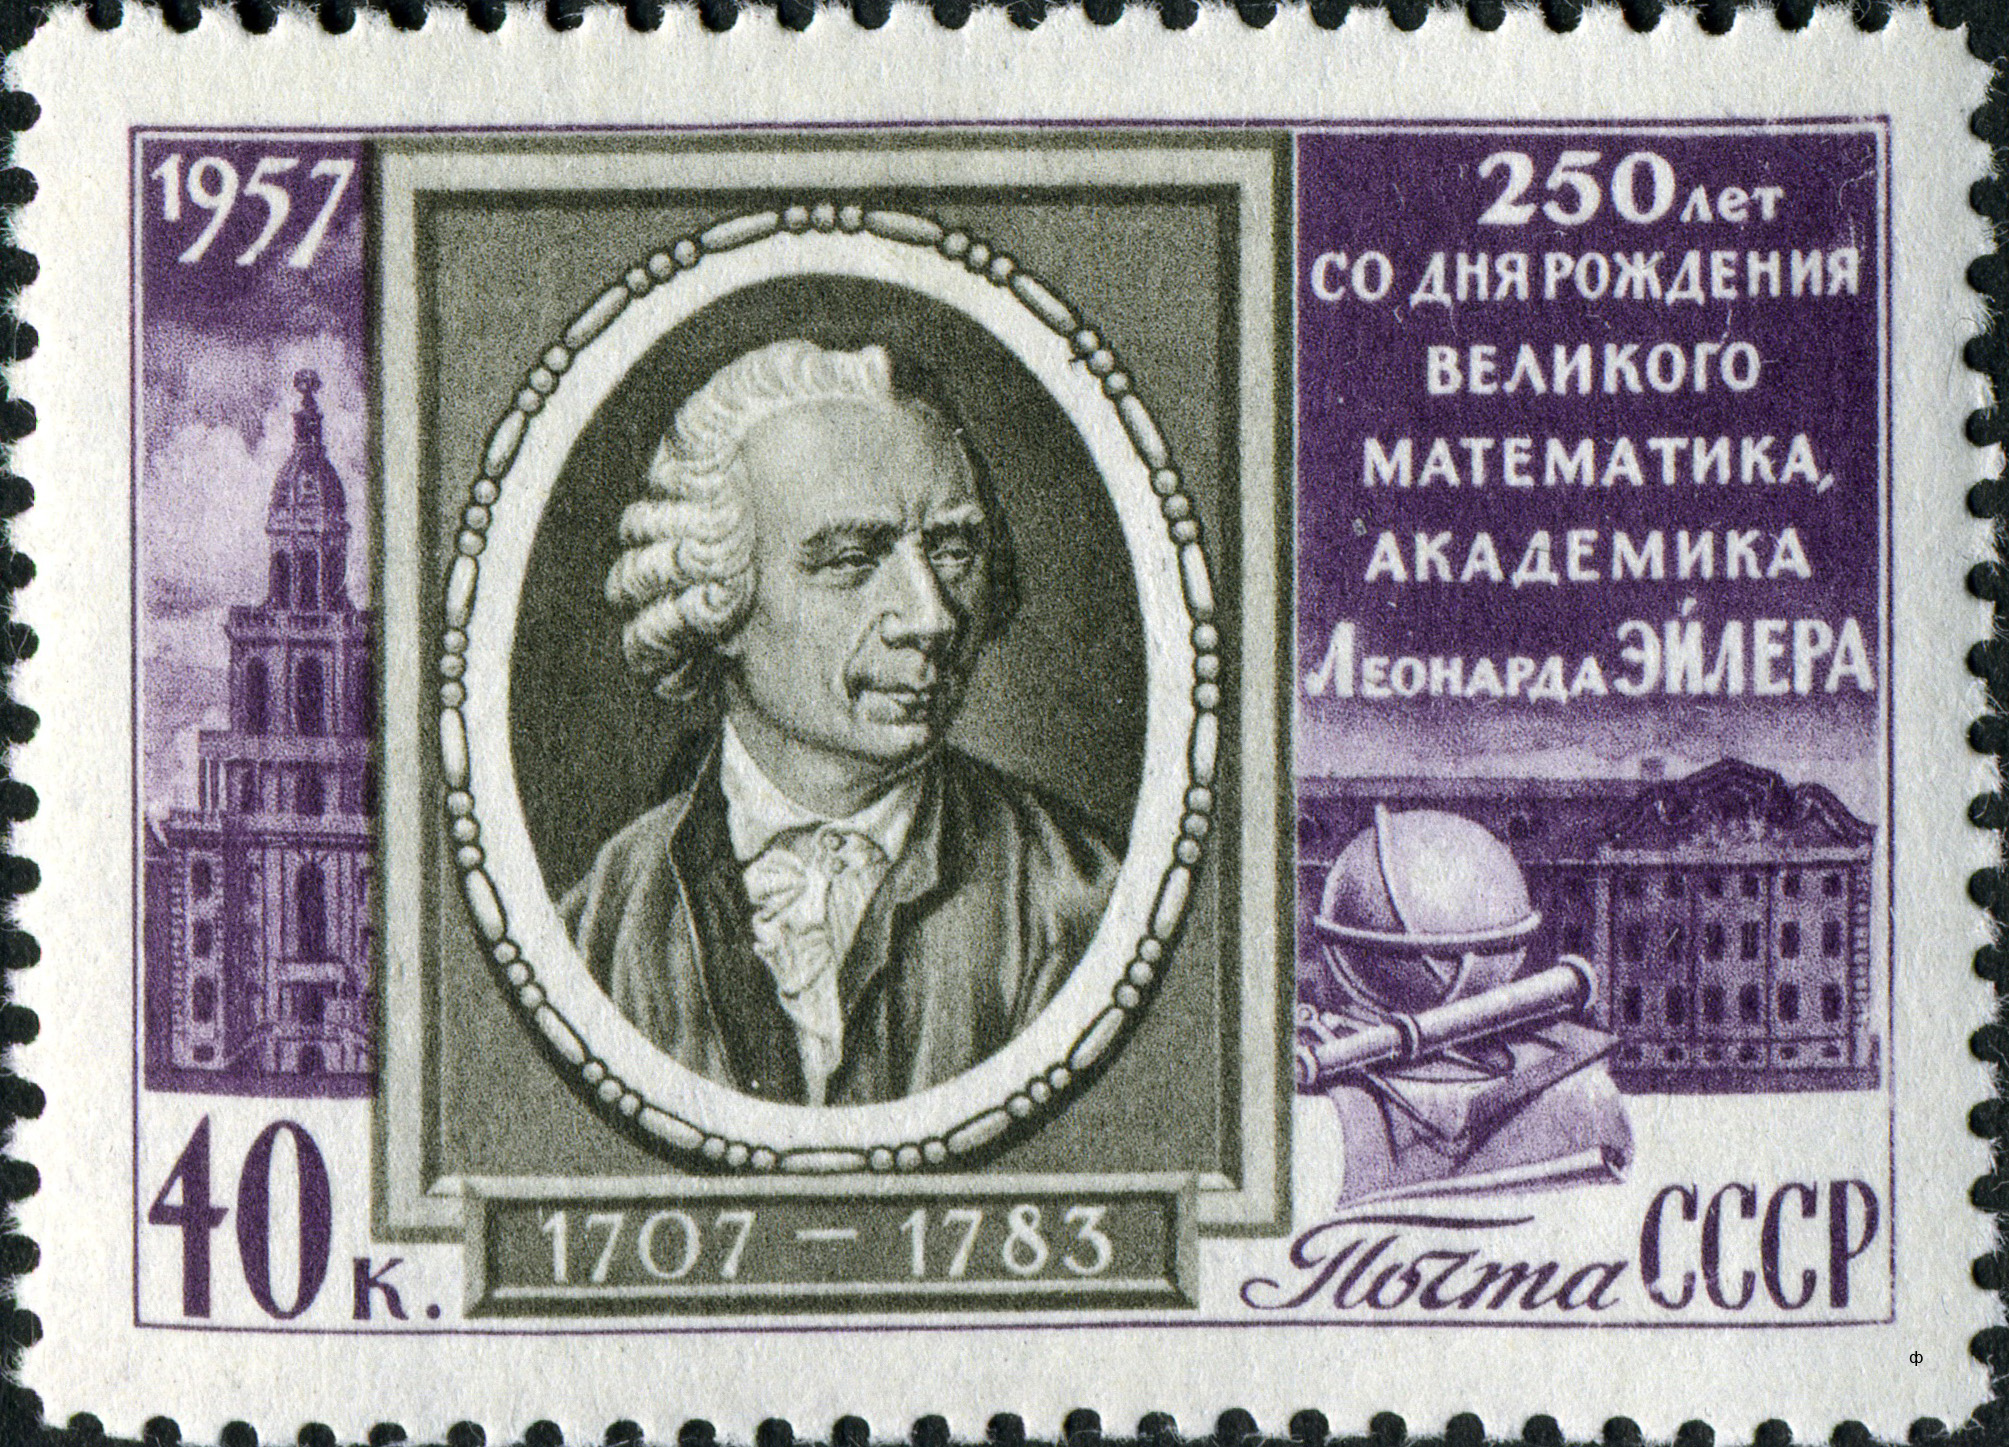
\includegraphics[height=5.2cm]{../mathematicians/Euler_Stamp.jpg} & 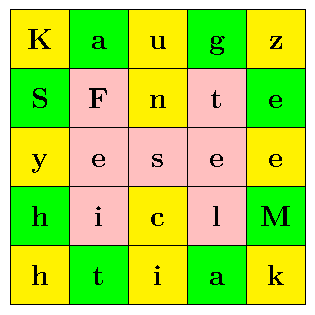
\includegraphics{./logo.pdf} \\
                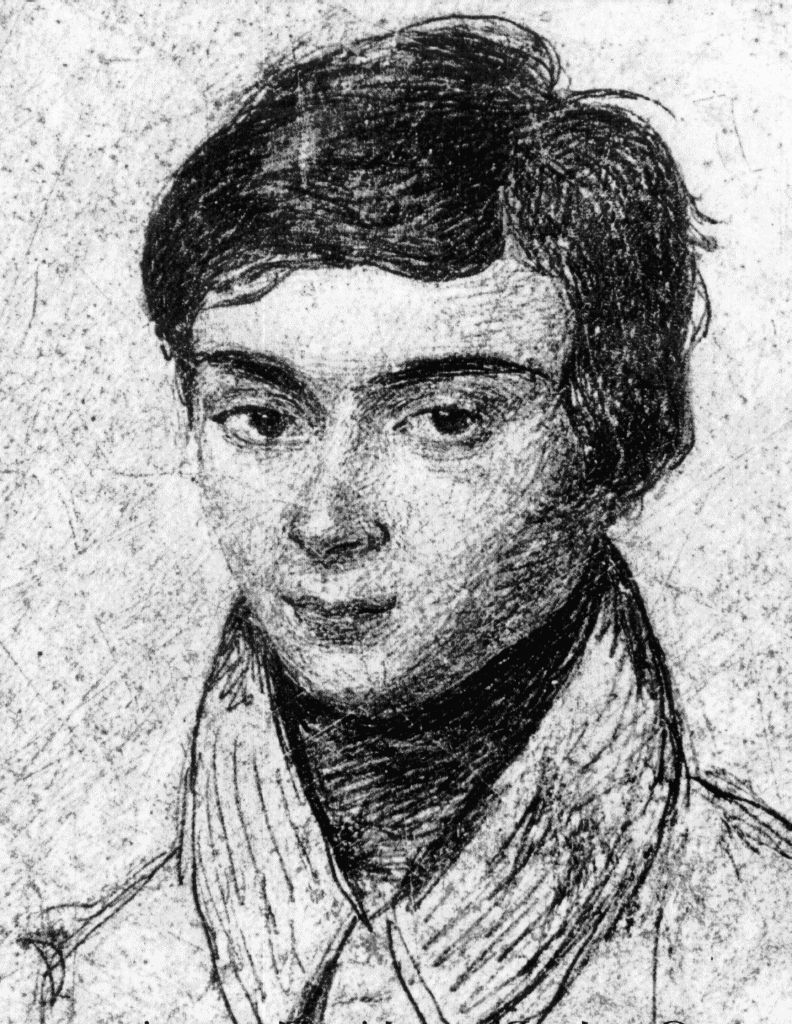
\includegraphics[height=5.2cm]{../mathematicians/Galois.jpg} & 
            
        \end{tabular}
    \end{center}
\end{titlepage}
\end{document}

\tableofcontents

\nomenclature{$\ZZ$}{Tập hợp số nguyên}
\nomenclature{$\QQ$}{Tập hợp số hữu tỷ}
\nomenclature{$\RR$}{Tập hợp số thực}
\nomenclature{$\CC$}{Tập hợp số phức}

\printnomenclature

\part{Đại số}

\subimport{algebra/}{algebra.tex}

\part{Đại số tuyến tính}

\parttoc

\chapter{Ma trận}

Trong các bài viết của về đại số tuyến tính:

\begin{itemize}
    \item Vector sẽ được ký hiệu bởi chữ thường in đậm (ví dụ $\bm{v}, \bm{x}, \ldots$)​; 
    \item Ma trận sẽ được ký hiệu bởi chữ hoa in đậm (ví dụ $\bm{A},\ \bm{B}, \ldots$​);
    \item Các đại lượng vô hướng (số) được ký hiệu bởi chữ thường không in đậm (ví dụ $x_1,\ N,\ t, \ldots$).
\end{itemize}

\begin{table}[htb]
    \caption{Thuật ngữ và ký hiệu}
    \begin{tabularx}{\textwidth}
        {|>{\raggedright\arraybackslash\hsize=0.2\textwidth}X|>{\raggedright\arraybackslash}X|}
        \hline
        \textbf{Ký hiệu} & \textbf{Ý nghĩa} \\ \hline\hline
        $\bm{A}^T$ & Ma trận chuyển vị (transpose) của ma trận $\bm{A}$ \\ \hline
        $\bm{A}^{-1}$ & Ma trận nghịch đảo (inverse) của ma trận $\bm{A}$ \\ \hline
        $\rank A$ & Hạng (rank) của ma trận $A$ \\ \hline
        $\det A$ & Định thức (determinant) ma trận $A$ \\ \hline
        $\bm{x} \cdot \bm{y}$ & Tích vô hướng hai vector $\bm{x}$ và $\bm{y}$ \\ \hline
        $\dim \mathcal{V}$ & Số chiều (dimension) không gian vector $\mathcal{V}$ \\ \hline
        $\lVert \bm{x} \rVert$ & Chuẩn Euclid (Euclidean norm) vector $\bm{x}$ \\ \hline
    \end{tabularx}
\end{table}

\section{Định thức, ma trận nghịch đảo, hạng ma trận}

\subsection*{Định thức ma trận}

\begin{definition}[Nghịch thế]
    Cho tập hợp $A = \{1, 2, \cdots, n\}$ và xét hoán vị $\sigma$ trên ​$A$. Ta gọi hai phần tử $i$​ và $j$​ tạo thành \textbf{nghịch thế} (inversion) nếu $i < j$​ và $\sigma(i) > \sigma(j)$.

    Đặt $\sigma = \{k_1, k_2, \cdots, k_n\}$​ là một hoán vị của $A$​. Ta ký hiệu \[ P\{k_1, k_2, \cdots, k_n\} \] là số lượng nghịch thế của $\sigma$​ và đặt \[ (-1)^{P\{k_1, k_2, \cdots, k_n\}} = \sign \{k_1, k_2, \cdots, k_n\}. \]
\end{definition}

\begin{example}
    Với $n=4$​, $A = \{1, 2, 3, 4\}$​. Xét hoán vị $\sigma = \{4, 2, 1, 3\}$.

    Ta nhận thấy các cặp nghịch thế $(4, 2),\ (4, 1),\ (4, 3),\ (2, 1)$​ gồm 4 cặp nghịch thế. Vậy $P\{4, 2, 1, 3\} = 4$ và $\sign \{4, 2, 1, 3\}=(-1)^4=1$​.
\end{example}

\begin{definition}[Định thức]
    Khi đó định thức của ma trận $\bm{A} = \begin{pmatrix}a_{11} & a_{12} & \cdots & a_{1n} \\ a_{21} & a_{22} & \cdots & a_{2n} \\ \cdots & \cdots & \cdots & \cdots \\ a_{n1} & a_{n2} & \cdots & a_{nn}\end{pmatrix}$ được định nghĩa là:
    \begin{equation}
        \det(\bm{A})=\displaystyle{\sum_{(i_1, i_2, \cdots, i_n)} a_{1, i_1} \cdot a_{2, i_2} \cdot a_{n, i_n} \cdot \sign\{i_1, i_2, \cdots, i_n\}}
    \end{equation}
    với mọi hoán vị $(i_1, i_2, \cdots, i_n)$ của $(1, 2, \cdots, n)$. Như vậy có $n!$​ phần tử cho tổng trên.
\end{definition}

\begin{example}
    Tính định thức ma trận $\bm{A}=\begin{pmatrix}1 & 2 & 3 \\ 4 & 5 & 6 \\ 7 & 8 & 9\end{pmatrix}$​.

    Xét hoán vị $\sigma_1 = \{1, 2, 3\}$​. Khi đó $P\{1, 2, 3\}=0$​, $a_{11} \cdot a_{22} \cdot a_{33} \cdot (-1)^0 = 1 \cdot 5 \cdot 9 \cdot 1 = 45$​.

    Xét hoán vị $\sigma_2 = \{1, 3, 2\}$​. Khi đó $P\{1, 3, 2\} = 1$​, $a_{11} \cdot a_{23} \cdot a_{32} \cdot (-1)^1 = 1 \cdot 6 \cdot 8 \cdot (-1) = -48$.

    Xét hoán vị $\sigma_3 = \{2, 1, 3\}$​. Khi đó $P\{2,1,3\}=1$​, $a_{12} \cdot a_{21} \cdot a_{33} \cdot (-1)^1 = 2 \cdot 4 \cdot 9 \cdot (-1) = -72$.

    Xét hoán vị $\sigma_4=\{2,3,1\}$. Khi đó $P\{2, 3, 1\} = 2$​, $a_{12} \cdot a_{23} \cdot a_{31} \cdot (-1)^2 = 2 \cdot 6 \cdot 7 \cdot 1 = 84$​.

    Xét hoán vị $\sigma_5=\{3, 1, 2\}$. Khi đó $P\{3, 1, 2\} = 2$​, $a_{13} \cdot a_{21} \cdot a_{32} \cdot (-1)^2 = 3 \cdot 4 \cdot 8 \cdot 1 = 96$​.

    Xét hoán vị $\sigma_6=\{3, 2, 1\}$​. Khi đó $P\{3, 2, 1\}=3$​, $a_{13} \cdot a_{22} \cdot a_{31} \cdot (-1)^3 = 3 \cdot 5 \cdot 7 \cdot  (-1) = -105$​.

    Như vậy $\det(A)=45-48-72+84+96-105=0$​.
\end{example}

Định thức của ma trận còn được định nghĩa theo \textbf{đệ quy} như sau:

Với ma trận $1 \times 1$ là $\bm{A}=\begin{pmatrix}a_{11}\end{pmatrix}$ thì $\det(\bm{A})=a_{11}$.

Với ma trận $2 \times 2$ là $\bm{A} = \begin{pmatrix}a_{11} & a_{12} \\ a_{21} & a_{22}\end{pmatrix}$​ thì $\det(\bm{A})=a_{11}a_{22} - a_{21}a_{12}$.

Với ma trận $n \times n$, gọi $\bm{M}_{ij}$ là ma trận có được từ ma trận $\bm{A}$ khi bỏ đi hàng $i$​ và cột $j$​ của ma trận $\bm{A}$ và ký hiệu $A_{ij}=(-1)^{i+j} \det (\bm{M}_{ij})$. Khi đó:

\begin{theorem}[Định lý Laplace]
    Định lý Laplace cho phép ta khai triển định thức của ma trận cấp $n$ thành tổng các ma trận cấp $n-1$.

    Khai triển theo cột $j$​: \[ \det(\bm{A})=\displaystyle{\sum_{i=1}^na_{ij} A_{ij}} = a_{1j} A_{1j} + a_{2j} A_{2j} + \cdots + a_{nj} A_{nj},\ j = \overline{1, n}.\]

    Khai triển theo hàng $i$​: \[ \det(\bm{A})=\displaystyle{\sum_{j=1}^n a_{ij} A_{ij}} = a_{i1} A_{i1} + a_{i2} A_{i2} + \cdots + a_{in} A_{in},\ i = \overline{1, n}. \]​
\end{theorem}

\subsection*{Ma trận nghịch đảo}

\begin{definition}[Ma trận nghịch đảo] 
    Ma trận $\bm{A}^{-1}$​ được gọi là \textbf{ma trận nghịch đảo} của ma trận vuông $\bm{A}$ nếu $\bm{A}^{-1} \cdot \bm{A} = \bm{A} \cdot \bm{A}^{-1} = \bm{I}$​. Trong đó $\bm{I}$ là ma trận đơn vị cùng kích thước với $\bm{A}$.
\end{definition}

\begin{equation}
    \bm{A}^{-1}=\frac{1}{\det(\bm{A})}[(A_{ij})_n]^T=\frac{1}{\det(\bm{A})}\begin{pmatrix} A_{11} & A_{21} & \cdots & A_{n1} \\ A_{12} & A_{22} & \cdots & A_{n2} \\ \cdots & \cdots & \cdots & \cdots \\ A_{1n} & A_{2n} & \cdots & A_{nn} \end{pmatrix}
\end{equation}
Trong đó, $A_{ij}$ cũng được định nghĩa tương tự như khi tính định thức bằng khai triển theo dòng hoặc cột. Gọi $\bm{M}_{ij}$ là ma trận có được từ ma trận $\bm{A}$ khi bỏ đi hàng $i$​ và cột $j$​ của ma trận $\bm{A}$ và ký hiệu $A_{ij}=(-1)^{i+j} \det (\bm{M}_{ij})$.

Như vậy, điều kiện cần và đủ để một ma trận có nghịch đảo là định thức khác 0.

\subsection*{Hạng của ma trận}

\begin{definition}[Hạng của ma trận]
    Cho ma trận $\mathbf{A}_{m \times n}$. \textbf{Hạng} của ma trận là cấp của ma trận con lớn nhất có định thức khác 0.
\end{definition}

Nghĩa là, một ma trận vuông mà là ma trận con (lấy một phần của ma trận ban đầu) kích thước $r \times r$ mà có định thức khác 0 và $r$ lớn nhất, thì hạng của ma trận khi đó là $r$. 

\begin{remark}
    Ma trận con kích thước $r \times r$ là ma trận con của ma trận kích thước $m \times n$ nên $r \leqslant \min(m, n)$.
\end{remark}

\begin{example}
    Ma trận $\bm{A} = \begin{pmatrix}
        1 & 2 & 3 \\ 2 & 4 & 6 \\ 1 & 2 & 4
    \end{pmatrix}$ có định thức $\det(\bm{A}) = 0$. 
    
    Nhưng ma trận con của $\bm{A}$ là $\bm{B} = \begin{pmatrix}2 & 3 \\ 2 & 4\end{pmatrix}$ (lấy dòng 1 và 3, lấy cột 2 và 3) có định thức $\det(\bm{B}) = 2 \neq 0$, do đó $r = \text{rank}(\bm{A}) = 2$ ($\text{rank}(\bm{A})$ nghĩa là hạng của $\bm{A}$).
\end{example}


\section{Tổ hợp tuyến tính}

Xét tập hợp các vector $\{\bm{v}_1, \bm{v}_2, \ldots, \bm{v}_d\}$ trên $\RR$.

\begin{definition}[Tổ hợp tuyến tính]
Với vector $\bm{x}$ bất kì thuộc $\RR$, nếu tồn tại các số thực $\alpha_1, \alpha_2, \ldots, \alpha_d \in \RR$ sao cho
\[\bm{x} = \alpha_1 \bm{v}_1 + \alpha_2 \bm{v}_2 + \ldots + \alpha_d \bm{v}_d\]
thì $\bm{x}$ được gọi là \textbf{tổ hợp tuyến tính} của các vector $\bm{v}_i$, $i = 1, 2, \ldots, d$.
\end{definition}

Ta thấy rằng vector không $\bm{0}$ là tổ hợp tuyến tính của mọi tập các vector $\bm{v}_i$.

Bây giờ ta xét tổ hợp tuyến tính
\[\alpha_1 \bm{v}_1 + \alpha_2 \bm{v}_2 + \ldots + \alpha_d \bm{v}_d = \bm{0}\]

\begin{definition}[Độc lập tuyến tính]
    Tập hợp các vector $\bm{v}_1$, $\bm{v}_2$, ..., $\bm{v}_d$ được gọi \textbf{độc lập tuyến tính} nếu
    chỉ có duy nhất trường hợp $\alpha_1 = \alpha_2 = \ldots = \alpha_d = 0$ thỏa tổ hợp tuyến tính trên.    
\end{definition}

\begin{definition}[Phụ thuộc tuyến tính]
    Tập các vector là phụ thuộc tuyến tính nếu không độc lập tuyến tính.
    Nói cách khác tồn tại ít nhất một phần tử $\alpha_i \neq 0$.
\end{definition}

\section{Không gian vector}

\subsection*{Không gian vector}

Xét tập hợp các vector $\mathcal{V}$ trên trường $\FF$.

Ta định nghĩa hai phép tính cộng và nhân trên các vector này.

\begin{itemize}[noitemsep]
    \item Phép cộng là một ánh xạ $\mathcal{V} \times \mathcal{V} \to \mathcal{V}$ sao cho
    với mọi $\bm{x}, \bm{y} \in \mathcal{V}$ thì $\bm{x} + \bm{y} \in \mathcal{V}$
    \item Phân nhân vô hướng là ánh xạ $\FF \times \mathcal{V} \to \mathcal{V}$ sao cho
    với mọi $\alpha \in \FF$ và $\bm{x} \in \mathcal{V}$ thì $\alpha \bm{x} \in \mathcal{V}$
\end{itemize}

Nói cách khác, phép cộng 2 vector và phép nhân vô hướng 1 số với vector cho kết quả vẫn nằm trong không gian vector đó.

Đồng thời, phép cộng và phép nhân vô hướng phải thỏa mãn các tính chất sau

\begin{enumerate}
    \item Tính giao hoán với phép cộng: với mọi $\bm{x}, \bm{y} \in \mathcal{V}$, $\bm{x} + \bm{y} = \bm{y} + \bm{x}$
    \item Tính kết hợp với phép cộng: với mọi $\bm{x}, \bm{y}, \bm{z} \in \mathcal{V}$, $\bm{x} + (\bm{y} + \bm{z}) = (\bm{x} + \bm{y}) + \bm{z}$
    \item Phần tử đơn vị của phép cộng: tồn tại vector không $\bm{0} \in \mathcal{V}$ sao cho với mọi $\bm{x} \in \mathcal{V}$, $\bm{0} + \bm{x} = \bm{x} + \bm{0} = \bm{x}$
    \item Phần tử đối của phép cộng: với mọi $\bm{x} \in \mathcal{V}$, tồn tại phần tử $\bm{x'} \in \mathcal{V}$ sao cho $\bm{x} + \bm{x'} = \bm{x} + \bm{x'} = \bm{0}$
    \item Phần tử đơn vị của phép nhân vô hướng: tồn tại phần tử $1_F \in \FF$ sao cho với mọi $\bm{x} \in \mathcal{V}$ thì $1_F \cdot \bm{x} = \bm{x}$
    \item Tính kết hợp của phép nhân vô hướng: với mọi $\alpha, \beta \in \FF$, với mọi $\bm{x} \in \mathcal{V}$ thì $\alpha (\beta \bm{x}) = (\alpha \beta) \bm{x}$
    \item Tính phân phối giữa phép cộng và nhân: với mọi $\alpha \in \FF$, với mọi $\bm{x}, \bm{y} \in \mathcal{V}$ thì $\alpha (\bm{x} + \bm{y}) = \alpha \bm{x} + \alpha \bm{y}$
    \item Tính phân phối giữa phép nhân vô hướng: với mọi $\alpha, \beta \in \FF$, với mọi $\bm{x} \in \mathcal{V}$ thì $(\alpha + \beta) \bm{x} = \alpha \bm{x} + \beta \bm{x}$
\end{enumerate}

Ta thấy rằng không gian vector ở chương trình phổ thông là không gian vector xác định trên trường $\FF = \RR$.
Khi đó $\mathcal{V} = \RR^n$. Trong chương này sẽ làm việc với không gian vector thực $\RR$.

\subsection*{Cơ sở và số chiều của không gian vector}

Nếu trong không gian vector $\mathcal{V}$ tồn tại các vector độc lập tuyến tính $\bm{v_1}$, $\bm{v_2}$, ..., $\bm{v_d}$
mà tất cả các vector trong $\mathcal{V}$ có thể biểu diễn dưới dạng tổ hợp tuyến tính của các vector $\bm{v_i}$ trên,
thì tập hợp các vector 
\[\{ \bm{v}_1, \bm{v}_2, \ldots, \bm{v}_d \}\]
được gọi là \textbf{cơ sở} của không gian vector $\mathcal{V}$.

Khi đó,
\[\bm{x} = \sum_{i=1}^{d} \alpha_i \bm{v}_i \quad \forall \bm{x} \in \mathcal{V}\]

Số lượng phần tử của tập hợp các vector đó (ở đây là $d$) gọi là \textbf{số chiều (dimension)} của không gian vector $\mathcal{V}$.
Ta ký hiệu $\text{dim} \mathcal{V} = d$.

Ta còn ký hiệu 
\[\mathcal{V} = \text{span} \{\bm{v}_1, \bm{v}_2, \ldots, \bm{v}_d\}\]
và nói là không gian vector $\mathcal{V}$ được span (hay được sinh) bởi các vector $\bm{v_i}$.

Ta thấy rằng có thể có nhiều cơ sở cho cùng một không gian vector.

\begin{theorem}
    Mọi cơ sở của không gian vector $\mathcal{V}$ đều có số phần tử bằng $\text{dim} \mathcal{V}$.
\end{theorem}

Giả sử ta có $\bm{v}_1$, $\bm{v}_2$, ..., $\bm{v}_d$ là một cơ sở của không gian vector $\RR^n$.
Khi đó nếu hệ vector $\bm{w}_1$, $\bm{w}_2$, ..., $\bm{w}_d$ cũng là một hệ cơ sở khi và chỉ khi tồn 
tại ma trận khả nghịch $\bm{A}$ sao cho $\bm{W} = \bm{A} \cdot \bm{V}$. Ở đây $\bm{W}$ là ma trận với các hàng là các vector $\bm{w}_i$. Tương tự $\bm{V}$ là ma trận với các hàng là các vector $\bm{v}_i$.

\begin{proof}
    Ta viết các vector $\bm{v}_i$ dưới dạng $\RR^n$.
    \begin{align*}
        \bm{v}_1 & = (v_{11}, v_{12}, \ldots, v_{1n}) \\
        \bm{v}_2 & = (v_{21}, v_{22}, \ldots, v_{2n}) \\
        \ldots & = (\ldots, \ldots, \ldots, \ldots) \\
        \bm{v}_d & = (v_{d1}, v_{d2}, \ldots, v_{dn})
    \end{align*}

    Tương tự là các vector $\bm{w}_i$.
    \begin{align*}
        \bm{w}_1 & = (w_{11}, w_{12}, \ldots, w_{1n}) \\
        \bm{w}_2 & = (w_{21}, w_{22}, \ldots, w_{2n}) \\
        \ldots & = (\ldots, \ldots, \ldots, \ldots) \\
        \bm{w}_d & = (w_{d1}, w_{d2}, \ldots, w_{dn})
    \end{align*}

    Do $\bm{v}_i$ là một cơ sở của $\RR^n$, mọi vector trong $\RR^n$ được biểu diễn dưới dạng tổ hợp tuyến tính của các $\bm{v}_i$.

    Khi đó ta viết các $\bm{w}_i$ dưới dạng tổ hợp tuyến tính của $\bm{v_i}$.
    \begin{align*}
        \bm{w}_1 & = \alpha_{11} \bm{v}_1 + \alpha_{12} \bm{v}_2 + \ldots + \alpha_{1d} \bm{v}_d \\
        \bm{w}_2 & = \alpha_{21} \bm{v}_1 + \alpha_{22} \bm{v}_2 + \ldots + \alpha_{2d} \bm{v}_d \\
        \ldots & = \ldots \\
        \bm{w}_d & = \alpha_{d1} \bm{v}_1 + \alpha_{d2} \bm{v}_2 + \ldots + \alpha_{dd} \bm{v}_d
    \end{align*}

    Điều này tương đương với 
    \begin{equation*}
        \begin{pmatrix}
            w_{11} & w_{12} & \ldots & w_{1n} \\
            w_{21} & w_{22} & \ldots & w_{2n} \\
            \ldots & \ldots & \ldots & \ldots \\
            w_{d1} & w_{d2} & \ldots & w_{dn}
        \end{pmatrix}
        = \begin{pmatrix}
            \alpha_{11} & \alpha_{12} & \ldots & \alpha_{1d} \\
            \alpha_{21} & \alpha_{22} & \ldots & \alpha_{2d} \\
            \ldots & \ldots & \ldots & \ldots \\
            \alpha_{d1} & \alpha_{d2} & \ldots & \alpha_{dd}
        \end{pmatrix}
        \times \begin{pmatrix}
            v_{11} & v_{12} & \ldots & v_{1n} \\ 
            v_{21} & v_{22} & \ldots & v_{2n} \\ 
            \ldots & \ldots & \ldots & \ldots \\ 
            v_{d1} & v_{d2} & \ldots & v_{dn}
        \end{pmatrix}
    \end{equation*}
    
    Nếu $\bm{w}_i$ cũng là cơ sở của $\mathcal{V}$, thì các vector $\bm{v}_i$ cũng phải
    biểu diễn được dưới dạng tổ hợp tuyến tính của $\bm{w}_i$.
    Nói cách khác, ma trận $(\alpha_{ij})$ khả nghịch và ta có điều phải chứng minh.
\end{proof}

\subsection*{Không gian vector con}

Cho không gian vector $\mathcal{V} \subset \RR^n$ với phép cộng hai vector
và phép nhân vô hướng. Một tập con $L$ của $\mathcal{V}$ được gọi
là không gian vector con nếu:

\begin{itemize}
    \item Với mọi $\bm{x}$, $\bm{y}$ thuộc $L$, $\bm{x} + \bm{y} \in L$
    \item Với mọi $\alpha \in \RR$, với mọi $\bm{x} \in L$, $\alpha \bm{x} \in L$
\end{itemize}

Nói cách khác, phép cộng và phép nhân vô hướng \textit{đóng} trong
không gian vector con.

\begin{remark}
    Trên $\RR^n$, hệ phương trình tuyến tính thuần nhất có thể sinh
    ra một không gian vector con của $\RR^n$.
\end{remark}

\begin{example}
    Xét hệ phương trình tuyến tính sau:
    \begin{equation*}
        \begin{array}{cccccccc}
            x_1 & + & 3x_2 & + & 5x_3 & + & 7x_4 & = 0 \\
            2x_1 & & & + & 4x_3 & + & 2x_4 & = 0 \\
            3x_1 & + & 2x_2 & + & 8x_3 & + & 7x_4 & = 0
        \end{array}
    \end{equation*}

    Biến đổi ma trận
    \begin{equation*}
        \begin{pmatrix}
            1 & 3 & 5 & 7 \\
            2 & 0 & 4 & 2 \\
            3 & 2 & 8 & 7
        \end{pmatrix} \sim \begin{pmatrix}
            1 & 3 & 5 & 7 \\
            0 & -6 & -6 & -12 \\
            0 & -7 & -7 & -14
        \end{pmatrix} \sim \begin{pmatrix}
            1 & 3 & 5 & 7 \\
            0 & 1 & 1 & 2 \\
            0 & 0 & 0 & 0
        \end{pmatrix}
    \end{equation*}

    Như vậy hệ tương đương với
    \[x_1 + 3x_2 + 5x_3 + 7x_4 = 0, \quad x_2 + x_3 + 2x_4 = 0\]

    Ta chọn $x_3, x_4 \in \RR$ tự do, khi đó $x_1$ và $x_2$ được 
    biểu diễn theo $x_3$ và $x_4$ 
    \begin{equation*}
        x_1 = -2x_3 - x_4, \quad x_2 = -x_3 - 2x_4
    \end{equation*}

    Mọi vector trong không gian tuyến tính khi đó có dạng
    \begin{align*}
        (x_1, x_2, x_3, x_4) & = (-2x_3 - x_4, -x_3 - 2x_4, x_3, x_4)
        \\ & = x_3 \cdot (-2, -1, 1, 0) + x_4 \cdot (-1, -2, 0, 1) 
    \end{align*}

    Ở đây ta thấy $x_3, x_4$ nhận giá trị tùy ý trong $\RR$, và
    mọi vector trong không gian nghiệm là tổ hợp tuyến tính của
    hai vector $(-2, -1, 1, 0)$ và $(-1, -2, 0, 1)$. Suy ra hai vector
    này là cơ sở của không gian nghiệm, và $\dim \mathcal{V} = 2$.

\end{example}

\section{Không gian Euclide}

Trên không gian vector $\mathcal{V}$ chúng ta bổ sung thêm một phép toán là tích vô hướng (dot product, tích chấm) của hai vector.

Giả sử với hai vector $\bm{x} = (x_1, x_2, \ldots, x_n)$ và $\bm{y} = (y_1, y_2, \ldots, y_n)$. Khi đó tích vô hướng của $\bm{x}$ và $\bm{y}$ là

\begin{equation}
	\bm{x} \cdot \bm{y} = x_1 y_1 + x_2 y_2 + \ldots + x_n y_n
\end{equation}

Một số sách ký hiệu tích vô hướng của hai vector $\bm{x}$ và $\bm{y}$ là $\langle \bm{x}, \bm{y} \rangle$. Trong quyển sách này mình sẽ dùng ký hiệu $\bm{x} \cdot \bm{y}$ như trên.

Không gian vector có phép toán tích vô hướng được gọi là không gian Euclide. Khi $\bm{x} = \bm{y}$ thì căn bậc hai của kết quả tích vô hướng được gọi là \textbf{chuẩn Euclide} (Euclidean norm) và được ký hiệu

\begin{equation}
	\lVert \bm{x} \rVert = \sqrt{\bm{x} \cdot \bm{x}} = \sqrt{x_1^2 + x_2^2 + \ldots + x_n^2}
\end{equation}

Như vậy ta có thể viết $\lVert \bm{x} \rVert^2 = \bm{x}^2$.

\begin{theorem}[Bất đẳng thức Cauchy-Schwarz]
	Với hai vector $\bm{x}$ và $\bm{y}$ bất kì ta luôn có
	
	\begin{equation}
		\lVert \bm{x} \rVert \cdot \lVert \bm{y} \rVert \geqslant \lvert \bm{x} \cdot \bm{y} \rvert
	\end{equation}
	
	Nghĩa là tích độ dài của hai vector bất kì trong cùng không gian Euclide lớn hơn hoặc bằng tích vô hướng giữa chúng. Dấu bằng xảy ra khi và chỉ khi $\dfrac{x_1}{y_1} = \dfrac{x_2}{y_2} = \ldots = \dfrac{x_n}{y_n}$. Nói cách khác là hai vector cùng phương.
\end{theorem}

\begin{proof}
	Với mọi số thực $t$, ta luôn có 
	\[0 \leqslant \lVert \bm{x} - t \bm{y} \rVert^2 = \bm{x}^2 - 2 t \bm{x} \cdot \bm{y} + t^2 \bm{y}^2 = \lVert \bm{x} \rVert^2 - 2 t \bm{x} \cdot \bm{y} + t^2 \lVert \bm{y} \rVert^2 \]
	
	Nếu xem biểu thức trên là đa thức bậc 2 theo $t$, để đa thức lớn hơn hoặc bằng 0 với mọi $t \in \RR$ thì ta phải có $\Delta' \leqslant 0$ và $\lVert \bm{y} \rVert^2 > 0$ (luôn đúng). Ta có
	\[\Delta' = (\bm{x} \cdot \bm{y})^2 - \lVert \bm{x} \rVert^2 \cdot \lVert \bm{y} \rVert^2 \leqslant 0 \]
	Tương đương với $\lvert \bm{x} \cdot \bm{y} \rvert \leqslant \lVert \bm{x} \rVert \cdot \lVert \bm{y} \rVert$ (điều phải chứng minh).
\end{proof}

\subsection*{Hệ cơ sở trực giao}

Cho không gian Euclide $\mathcal{V}$ và một cơ sở của nó là $\bm{v}_1$, $\bm{v}_2$, ..., $\bm{v}_d$. Thuật toán trực giao Gram-Schmidt là thuật toán biến đổi cơ sở trên thành một cơ sở mới, trong đó các vector đều trực giao nhau.

\begin{algorithm}
	\caption{Thuật toán trực giao Gram-Schmidt}
	\begin{algorithmic}
		\Require $\bm{v}_1$, ..., $\bm{v}_d$ trong $\RR^n$
		\Ensure $\bm{u}_1$, ..., $\bm{u}_d$ trong $\RR^n$ mà $\bm{u}_i \cdot \bm{u}_j = 0$ với mọi $i \neq j$
		\State $\bm{u}_1 \gets \bm{v}_1$
		\For{$i = 2 \to d$}
			\State $\bm{w} = \bm{v}_i$
			\For{$j = i-1 \to 1$}
			\State $\mu_{i,j} = (\bm{v}_i \cdot \bm{u}_j) / (\bm{u}_i \cdot \bm{u}_j)$
			\State $\bm{w} \gets \bm{w} - \mu_{i, j} \bm{u}_j$
			\EndFor
			\State $\bm{u}_i \gets \bm{w}$
		\EndFor
		\State \Return $\bm{u}_1$, ..., $\bm{u}_d$
	\end{algorithmic}
\end{algorithm}

Nói cách khác, với $\bm{u}_1 = \bm{v}_1$, với mỗi $i = 2, 3, \ldots, d$ ta tính vector $\bm{u}_i$ với công thức
\begin{equation*}
	\bm{u}_i = \bm{v}_i - \sum_{j=1}^{i-1} \mu_{i,j} \bm{u}_j
\end{equation*}

Ở đây $\mu_{i,j} = \dfrac{\bm{v}_i \cdot \bm{u}_j}{\bm{u}_i \cdot \bm{u}_j}$ là hệ số trước $\bm{u}_j$.

\begin{example}
	Xét cơ sở $\bm{v}_1 = (2, -2, 4)$, $\bm{v}_2 = (1, -1, 0)$ và $\bm{v}_3 = (5, -3, 3)$ của $\RR^3$.
	
	Đặt $\bm{u}_1 = \bm{v}_1 = (2, -2, 4)$.
	
	Ta có $\mu_{2,1} = \dfrac{\bm{v}_2 \cdot \bm{u}_1}{\bm{u}_1 \cdot \bm{u}_1} = \dfrac{1 \cdot 2 + (-1) \cdot (-2) + 0 \cdot 4}{2^2 + (-2)^2 + 4^2} = \dfrac{4}{24} = \dfrac{1}{6}$.
	
	Suy ra \[\bm{u}_2 = \bm{v_2} - \mu_{2, 1} \bm{u}_1 = (1, -1, 0) - \dfrac{1}{6} \cdot (2, -2, 4) = \Bigl(\dfrac{2}{3}, \dfrac{-2}{3}, \dfrac{-2}{3}\Bigr)\]
	
	Tương tự $\mu_{3, 1} = \dfrac{\bm{v}_3 \cdot \bm{u}_1}{\bm{u}_1 \cdot \bm{u}_1} = \dfrac{5 \cdot 2 + (-3) \cdot (-2) + 3 \cdot 4}{2^2 + (-2)^2 + 4^2} = \dfrac{28}{24} = \dfrac{7}{6}$.
	
	Tiếp theo $\mu_{3,2} = \dfrac{\bm{v}_3 \cdot \bm{u}_2}{\bm{u}_2 \cdot \bm{u}_2} = \dfrac{5 \cdot \dfrac{2}{3} + (-3) \cdot \dfrac{-2}{3} + 3 \cdot \dfrac{-2}{3}}{ \Bigl(\dfrac{2}{3}\Bigr)^2 + \Bigl(\dfrac{-2}{3}\Bigr)^2 + \Bigl(\dfrac{-2}{3}\Bigr)^2 } = \dfrac{5}{2}$.
	
	\begin{align*}
		\Rightarrow \quad \bm{u}_3 = & \bm{v}_3 - \mu_{3,1} \bm{u}_1 - \mu_{3,2} \bm{u}_2 \\ = & (5, -3, 3) - \dfrac{7}{6} \cdot (2, -2, 4) - \dfrac{5}{2} \cdot \Big(\dfrac{2}{3}, \dfrac{-2}{3}, \dfrac{-2}{3}\Big) \\ = & (1, 1, 0)
	\end{align*}
	
	Ta có thể kiếm chứng rằng $\bm{u}_1 \cdot \bm{u}_2 = 2 \cdot \dfrac{2}{3} + (-2) \cdot \dfrac{-2}{3} + 4 \cdot \dfrac{-2}{3} = 0$. Tương tự với $\bm{u}_1 \cdot \bm{u}_3 = 0$ và $\bm{u}_2 \cdot \bm{u}_3 = 0$. Thêm nữa các vector này cũng độc lập tuyến tính nên cũng là một hệ cơ sở của $\RR^3$.
	
	Như vậy các vector $\bm{u}_1$, $\bm{u}_2$, $\bm{u}_3$ là một cơ sở trực giao của $\RR^3$.
\end{example}

\begin{remark}
	Cơ sở trực giao cho phép ta tính độ dài của tất cả các vector khác trong không gian vector dễ dàng hơn.
\end{remark}

Thật vậy, giả sử $\bm{u}_1$, $\bm{u}_2$, ..., $\bm{u}_d$ là các vector trong cơ sở trực giao. Mọi vector $\bm{x}$ trong không gian vector đều có dạng\[\bm{x} = \alpha_1 \bm{u}_1 + \alpha_2 \bm{u}_2 + \ldots + \alpha_d \bm{u}_d\]

Khi đó
\begin{align*}
    \lVert \bm{x} \rVert^2 = \bm{x}^2 = (\alpha_1 \bm{u}_1 + \alpha_2 \bm{u}_2 + \ldots + \alpha_d \bm{u}_d)^2 = \sum_{i=1}^d \alpha_i^2 \bm{u}_i^2 + 2 \sum_{i \neq j} \bm{u}_i \bm{u}_j
\end{align*}

Do các vector trong cơ sở đều trực giao với nhau nên $\bm{u}_i \cdot \bm{u}_j = 0$ với $i \neq j$, $1 \leqslant i, j \leqslant d$. Từ đó ta có được \[\lVert \bm{x} \rVert^2 = \sum_{i=1}^d \alpha_i^2 \bm{u}_i^2 = \sum_{i=1}^d \alpha_i^2 \lVert \bm{u}_i \rVert^2\] hay \[\lVert \bm{x} \rVert = \sqrt{\alpha_1^2 \bm{u}_1^2 + \ldots + \alpha_d^2 \bm{u}_d^2}\]

Kết quả rất đơn giản, độ dài của các vector bất kì là căn bậc hai của tổ hợp độ dài các vector trong cơ sở và hệ số tương ứng.

\subsection*{Chứng minh thuật toán Gram-Schmidt}

Cho không gian vector $\mathcal{V}$ với cơ sở là các vector $\bm{v}_1$, ..., $\bm{v}_d$. Thuật toán Gram-Schmidt biến đổi và cho kết quả là cơ sở mới $\bm{u}_1$, ..., $\bm{u}_d$ sao cho các vector trong cơ sở mới này trực giao nhau đôi một.

Đặt $\bm{u}_1 = \bm{v}_1$. 

\textbf{Bước 1}. Ta chứng minh với mọi $k \geqslant 2$ thì $\bm{u}_k \cdot \bm{u}_1 = 0$.

Ta có $\bm{u}_2 = \bm{v}_1 - \mu_{2, 1} \bm{u_1} = \bm{v}_2 - \dfrac{\bm{v}_2 \cdot \bm{u}_1}{\bm{u}_1 \cdot \bm{u}_1} \cdot \bm{u}_1$. 

Suy ra $\bm{u}_2 \cdot \bm{u}_1 = \bm{v}_2 \cdot \bm{u}_1 - \dfrac{\bm{v}_2 \cdot \bm{u}_1}{\bm{u}_1 \cdot \bm{u}_1} \cdot (\bm{u}_1 \cdot \bm{u}_1) = \bm{v}_2 \cdot \bm{u}_1 - \bm{v}_2 \cdot \bm{u}_1 = 0$.

Như vậy với $k = 2$ thì đẳng thức đúng. Giả sử đẳng thức $\bm{u}_k \cdot \bm{u}_1 = 0$ đúng tới $k \geqslant 2$. Xét $k+1$ ta có
\[\bm{u}_{k+1} = \bm{v}_{k+1} - \sum_{j=1}^{k} \mu_{k+1, j} \bm{u}_j\]

Suy ra
\[\bm{u}_{k+1} \cdot \bm{u}_1 = \bm{v}_{k+1} \cdot \bm{u}_1 - \sum_{j=1}^{k} \dfrac{\bm{v}_{k+1} \cdot \bm{u}_j}{\bm{u}_j \cdot \bm{u}_j} \cdot (\bm{u}_j \cdot \bm{u}_1 )\]

Ta thấy rằng với $j = 2, \ldots, k$ thì $\bm{u}_j \cdot \bm{u}_1 = 0$ theo giả thiết quy nạp. Như vậy chỉ còn lại $j = 1$ và kết quả là
\[\bm{u}_{k+1} \cdot \bm{u}_1 = \bm{v}_{k+1} \cdot \bm{u}_1 - \dfrac{\bm{v}_{k+1} \cdot \bm{u}_1}{\bm{u}_1 \cdot \bm{u}_1} \cdot (\bm{u}_1 \cdot \bm{u}_1) = 0\]

\textbf{Bước 2}. Ta chứng minh với mọi $k \geqslant 3$ thì $\bm{u}_k \cdot \bm{u}_2 = 0$.

Tương tự ta sử dụng quy nạp. Ta có $\bm{u}_3 = \bm{v}_3 - \mu_{3,2} \bm{u}_2 - \mu_{3,1} \bm{u}_1$. Suy ra $\bm{u}_3 \cdot \bm{u}_2 = \bm{v}_3 \cdot \bm{u}_2 - \mu_{3,2} \bm{u}_2 \cdot \bm{u}_2 - \mu_{3,1} \cdot \bm{u}_1 \cdot \bm{u}_2$. Ta đã chứng minh được $\bm{u}_2 \cdot \bm{u}_1 = 0$. Như vậy kết quả sẽ là
\[\bm{u}_3 \cdot \bm{u}_2 = \bm{v}_3 \cdot \bm{u}_2 - \dfrac{\bm{v}_3 \cdot \bm{u}_2}{\bm{u}_2 \cdot \bm{u}_2} \cdot (\cdot \bm{u}_2 \cdot \bm{u}_2) = 0\]

Với giả thiết quy nạp $\bm{u}_k \cdot \bm{u}_2 = 0$ đúng tới $k \geqslant 3$, ta xét $k+1$. Khi đó
\[\bm{u}_{k+1} = \bm{v}_{k+1} - \sum_{j=1}^k \mu_{k+1,j} \bm{u}_j\]

Suy ra
\[\bm{u}_{k+1} \cdot \bm{u}_2 = \bm{v}_{k+1} \cdot \bm{u}_2 - \sum_{j=1}^k \mu_{k+1,j} \bm{u}_j \cdot \bm{u}_2\]

Theo giả thiết quy nạp thì mọi $j \geqslant 3$ đều cho kết quả $\bm{u}_j \cdot \bm{u}_2 = 0$, thêm nữa là $\bm{u}_1 \cdot \bm{u}_2 = 0$ do chứng minh trên. Như vậy trong tổng chỉ còn lại $j=2$ và kết quả sẽ là
\[\bm{u}_{k+1} \cdot \bm{u}_2 = \bm{v}_{k+1} \cdot \bm{u}_2 - \dfrac{\bm{v}_{k+1} \cdot \bm{u}_2}{\bm{u}_2 \cdot \bm{u}_2} \cdot (\bm{u}_2 \cdot \bm{u}_2) = 0\]

Từ đây có thể thấy, sử dụng phương pháp quy nạp ta có thể chứng minh được rằng với mỗi số $n \geqslant 2$, thì mọi $k \geqslant n+1$ ta đều có $\bm{u}_k \cdot \bm{u}_n = 0$. Hay nói cách khác là khi thuật toán tính $\bm{u}_k$ thì nó sẽ trực giao với tất cả $\bm{u}_1$, $\bm{u}_2$, ..., $\bm{u}_{k-1}$.

\part{Toán rời rạc}

\parttoc

\subimport{discrete_mathematic/}{discrete_logarithm}

\subimport{discrete_mathematic/}{relationship}

\subimport{discrete_mathematic/}{group.tex}

\subimport{discrete_mathematic/}{number_theory.tex}

\subimport{boolean/}{boolean_function.tex}

\subimport{discrete_mathematic/}{galois_theory.tex}

\part{Giải tích}

\parttoc

\chapter{Giải tích}

\begin{figure}[ht]
    \centering
    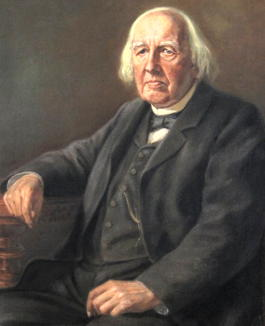
\includegraphics{mathematicians/Weiertrass.jpg}
    \captionsetup{labelformat=empty}
    \caption{Karl Theodor Wilhelm Weierstrass (1815-1897)}
\end{figure}

\section{Giới hạn}

\subsection*{Giới hạn của dãy số}

\begin{definition}[Giới hạn hữu hạn của dãy số]
    Cho dãy số $\{ a_n \}$. Ta nói dãy $\{ a_n \}$ có giới hạn hữu hạn $L$ nếu với mọi $\varepsilon > 0$, tồn tại $n_0 \in \NN$ sao cho với mọi $n \geqslant n_0$ thì 
    \begin{equation*}
        | a_{n} - L | < \varepsilon
    \end{equation*}

    Ký hiệu: $\displaystyle{\lim_{n \to \infty} a_n = L}$.
\end{definition}

\begin{example}
    Xét dãy số cho bởi công thức $a_n = \dfrac{1}{n}$. Ta chứng minh dãy số có giới hạn hữu hạn là 0.

    Với mọi $\varepsilon > 0$ tùy ý, ta cần chứng minh tồn tại số $n_0 \geqslant 1$ sao cho với mọi $n \geqslant n_0$ thì $| a_n - 0 | < \varepsilon$.

    Nói cách khác $a_{n_0} < \varepsilon$, hay tương đương với $\dfrac{1}{n_0} < \varepsilon \Leftrightarrow n_0 > \frac{1}{\varepsilon}$.

    Vậy ta chỉ cần chọn $n_0$ thỏa bất đẳng thức trên (luôn tìm được).

    Kết luận: $\displaystyle{\lim_{n \to \infty} a_n = 0}$
\end{example}

\begin{definition}[Dãy số có giới hạn vô cực]
    Cho dãy số $\{a_n\}$. Ta nói dãy số có giới hạn ở dương vô cực nếu với mọi $M > 0$, tồn tại $n_0 \in \NN$ sao cho với mọi $n \geqslant n_0$ thì $a_n > M$.
\end{definition}

Nói cách khác, nếu ta chọn một số $M$ rất lớn bất kì, thì mọi số hạng của dãy số kể từ một số hạng nào đó trở đi luôn lớn hơn $M$. Định nghĩa về dãy số có giới hạn ở âm vô cực cũng tương tự.

\subsection*{Giới hạn của hàm số}

Để định nghĩa giới hạn của hàm số $y = f(x)$ khi $x$ tiến tới $x_0$ ta có hai loại định nghĩa.

\begin{definition}[Giới hạn hàm số qua giới hạn dãy số]
    Xét hàm số $f(x)$. Ta nói hàm số có giới hạn hữu hạn $L$ khi $x$ tiến tới $x_0$, nếu với mọi dãy số $\{x_n\}$ mà $\displaystyle{\lim_{n \to \infty} x_n = x_0}$, thì  $\displaystyle{\lim_{n \to \infty} f(x_n) = L}$.
\end{definition}

Định nghĩa này tuân theo giới hạn của dãy số. Khi đó mọi phần tử của dãy số từ một số hạng nào đó trở đi cho giá trị $f(x_n)$ tiến về $L$.

Định nghĩa của hàm số theo kiểu Cauchy (hay còn được gọi là ngôn ngữ $\delta-\varepsilon$) là kiểu định nghĩa phổ biến được giảng dạy trong nhà trường.

\begin{definition}[Giới hạn hàm số kiểu Cauchy]
    Xét hàm số $f(x)$. Ta nói hàm số có giới hạn hữu hạn $L$ khi $x$ tiến tới $x_0$, nếu với mọi $\varepsilon > 0$, tồn tại  $\delta > 0$ sao cho với mọi $x$ mà $| x - x_0 | < \delta$ thì $|f(x) - L| < \varepsilon$.

    Ký hiệu: $\displaystyle{\lim_{x \to x_0} f(x) = L}$
\end{definition}

%Một cách hình ảnh, tương tự như giới hạn dãy số, lần này ta nhìn trên 2 trục  của mặt phẳng tọa độ $Oxy$. Với mọi quả cầu bán kính $\varepsilon$ tâm $L$ (dành cho $f(x)$) ta luôn chọn được quả cầu bán kính $\delta$ tâm $x_0$ (dành cho $x$). Lúc này khi $x$ nằm trong quả cầu tâm $x_0$ bán kính $\delta$ thì $f(x)$ tương ứng sẽ nằm trong quả cầu tâm $L$ bán kính $\varepsilon$.

Ta có thể thấy ở đây $x$ tiến về $x_0$ (khá giống định nghĩa giới hạn hàm số) và $f(x)$ tương ứng tiến về $L$.

Tương tự ta cũng có giới hạn hàm số ở vô cực.

\begin{definition}[Giới hạn hàm số ở vô cực]
    Với hàm số $f(x)$, ta nói hàm số có giới hạn tại dương vô cực khi $x$ tiến về $x_0$ nếu với mọi $M > 0$, tồn tại $\delta > 0$ sao cho với mọi $x$ mà $|x - x_0| < \delta$ thì $f(x) > M$.

    Ký hiệu: $\displaystyle{\lim_{x \to x_0} f(x) = +\infty}$.
\end{definition}

\begin{definition}[Giới hạn một bên]
    Ta nói hàm số $f(x)$ có giới hạn phải $L$ tại $x_0$ khi $x$ tiến về bên phải $x_0$ nếu với mọi $\varepsilon > 0$, tồn tại $\delta > 0$ sao cho với mọi $0 < x - x_0 < \delta$  thì $|f(x) - L| < \varepsilon$.

    Ký hiệu: $\displaystyle{\lim_{x \to x_0^+} f(x) = L}$
\end{definition}

Nghĩa là chúng ta chỉ xét giới hạn khi $x$ tiến tới $x_0$ từ bên phải $x > x_0$. Tương tự cho giới hạn trái.

Lưu ý rằng trong nhiều trường hợp, mặc dù cùng tiến tới $x_0$ nhưng giới hạn trái và giới hạn phải có thể không bằng nhau.

\begin{example}
    Xét hàm số $y = \frac{1}{x}$. Ta thấy hàm số không xác định tại $x = 0$, và giới hạn trái và phải khác nhau do \[\lim_{x \to 0^+} = +\infty, \quad \lim_{x \to 0^-} = -\infty\]
\end{example}

\subsection*{Tính liên tục của hàm số}

Cho hàm số $f(x)$ xác định trên miền $D$ và $x_0$ là một điểm thuộc $D$.

\begin{definition}[Hàm số liên tục tại một điểm]
    Ta nói hàm số $f(x)$ liên tục tại $x_0$ nếu \[\lim_{x \to x_0} f(x) = f(x_0)\]
\end{definition}

Định nghĩa tương tự cho liên tục trái và liên tục phải (ta lấy giới hạn một bên).

Như vậy, có 3 khả năng hàm số không liên tục tại một điểm.

\begin{enumerate}[noitemsep]
    \item Hàm số không xác định tại $x_0$
    \item Hàm số xác định tại $x_0$ nhưng giới hạn tại đó không bằng $f(x_0)$
    \item Giới hạn trái và giới hạn phải không bằng nhau
\end{enumerate}

Nếu hàm số không liên tục tại $x_0$ ta gọi hàm số bị \textbf{gián đoạn} tại $x_0$.

Nếu hàm số liên tục tại mọi điểm trên khoảng $(a, b)$ thì ta nói hàm số liên tục trên khoảng đó.

\section{Đạo hàm}

\begin{definition}[Đạo hàm]
    Cho hàm số $f(x)$ xác định trên miền $D$ và $x_0$ là điểm thuộc $D$. Ta nói hàm số $f(x)$ có đạo hàm tại $x_0$ (hoặc khả vi tại $x_0$) nếu tồn tại giới hạn hữu hạn
    \[\lim_{x \to x_0}\frac{f(x) - f(x_0)}{x - x_0}\]

    Ký hiệu đạo hàm của $f$ tại $x_0$ là $f'(x_0)$.
\end{definition}

\begin{example}
    Xét hàm số $f(x) = x^2 + 1$ trên $\RR$. Tìm đạo hàm tại $x_0 \in \RR$.

    Ta có $f(x)-f(x_0) = x^2 + 1 - (x_0^2 + 1) = (x - x_0) (x + x_0)$.

    Khi đó $\frac{f(x)-f(x_0)}{x-x_0} = x + x_0$ nên ta có $\displaystyle{\lim_{x \to x_0} (x + x_0) = 2 x_0}$.
\end{example}

Nếu hàm số khả vi trên mọi điểm thuộc khoảng (đoạn) nào đó thì ta nói hàm số khả vi trên khoảng (đoạn) đó và ký hiệu là $f'(x)$.

Với ví dụ trên, ta thấy giới hạn tồn tại với mọi $x_0 \in \RR$ nên ta có thể thay $x_0$ bởi $x$ và có $f'(x) = 2x$ với $f(x) = x^2 + 1$.

\begin{remark}
    Từ định nghĩa ta thấy rằng nếu $f(x)$ khả vi tại $x_0$ thì nó cũng liên tục tại $x_0$. Tuy nhiên chiều ngược lại không đúng. Ví dụ với hàm số $y = \lvert x \rvert$, hàm số liên tục tại $x=0$ nhưng giới hạn (đạo hàm) phải là 1, còn giới hạn (đạo hàm) trái là -1.
\end{remark}

Về mặt hình ảnh, khi hàm số khả vi tại một điểm thì đồ thị sẽ "trơn", không gấp khúc tại điểm đó.

\subsection*{Cực trị}

Đầu tiên chúng ta cần một định lý về tính đơn điệu của hàm số
khả vi.

\begin{theorem}
    Xét hàm số $f(x)$ khả vi trên khoảng $(a, b)$. Nếu $f'(x) > 0$ 
    với mọi $x \in (a, b)$ thì $f(x)$ đồng biến trên $(a, b)$.
\end{theorem}

Tương tự, $f'(x) < 0$ với mọi $x \in (a, b)$ thì $f(x)$ nghịch biến trên
$(a, b)$.

\begin{definition}[Cực tiểu của hàm số]
    Xét hàm số $f(x)$ liên tục trên khoảng $(a, b)$. Điểm $(x_0, f(x_0))$ được
    gọi là \textbf{cực tiểu} của hàm số $f(x)$ nếu tồn tại một lân cận $U$
    chứa $x_0$ nằm trong khoảng $(a, b)$ sao cho với mọi $x \in U$ thì $f(x) \geqslant f(x_0)$.
\end{definition}

\begin{definition}[Cực đại của hàm số]
    Xét hàm số $f(x)$ liên tục trên khoảng $(a, b)$. Điểm $(x_0, f(x_0))$ được
    gọi là \textbf{cực đại} của hàm số $f(x)$ nếu tồn tại một lân cận $U$
    chứa $x_0$ nằm trong khoảng $(a, b)$ sao cho với mọi $x \in U$ thì $f(x) \leqslant f(x_0)$.
\end{definition}

Theo định nghĩa cực tiểu thì chỉ cần tồn tại lân cận chứa $x_0$
mà $f(x) \geqslant f(x_0)$ thì điểm đó là cực tiểu. Như vậy một hàm số có 
thể có nhiều cực tiểu, tương tự cũng có thể có nhiều cực đại.

Lưu ý rằng cực đại và cực tiểu không phải điểm chỉ giá trị lớn nhất
hay giá trị nhỏ nhất của hàm số. Nó chỉ lớn nhất hoặc nhỏ nhất trong
vùng lân cận đó theo định nghĩa, nên người ta còn gọi là cực trị địa phương.

%Xét hàm số $f(x)$ khả vi trên khoảng $(a, b)$. Gọi $f'(x)$ là
%đạo hàm của hàm số $f(x)$ trên $(a, b)$. Khi đó điểm $x_0 \in (a, b)$ được gọi là
%\begin{itemize}
 %   \item Cực tiểu nếu $f'(x)$ đổi chiều từ âm sang dương khi đi qua $x_0$
 %   \item Cực đại nếu $f'(x)$ đổi chiều từ dương sang âm khi đi qua $x_0$
%\end{itemize}

\begin{definition}[Dãy Cauchy]
    Dãy $(x_n)$ được gọi là dãy Cauchy nếu với mọi $\varepsilon > 0$, tồn tại $N_0 \in \NN$ sao cho, với mọi $m, n > N_0$ thì $\lvert x_m - x_n \rvert < \varepsilon$.
\end{definition}

\begin{theorem}[Tiêu chuẩn Cauchy]
    Dãy số $(x_n)$ có giới hạn hữu hạn khi và chỉ khi nó là dãy Cauchy.
\end{theorem}

\begin{theorem}[Bổ đề Fermat]
    Cho $f$ là một hàm số có đạo hàm trên $(a, b)$. Nếu $x_0 \in (a, b)$ là một điểm cực trị của $f$ thì ta có $f'(x_0) = 0$.
\end{theorem}

\begin{proof}
    Ta chứng minh trong trường hợp $x_0$ là điểm cực tiểu. Trường hợp điểm cực đại tương tự.

    Hàm $f$ có đạo hàm trên $(a, b)$ nên tại điểm $x_0$ nó có đạo hàm bên trái và đạo hàm bên phải, và hai đạo hàm này bằng nhau.

    Ta có $\displaystyle{f'(x_0^+) = \lim_{x \to x_0^+} \frac{f(x) - f(x_0)}{x - x_0}}$. Vì $x \to x_0^+$ nghĩa là $x > x_0$ ($x$ tiến tới $x_0$ từ bên phải), và do $x_0$ là cực tiểu $f(x) - f(x_0) \geqslant 0$ nên phân số dưới dấu giới hạn lớn hơn 0. Suy ra $f'(x_0^+) \geqslant 0$.

    Hoàn toàn tương tự ta chứng minh được $f'(x_0^-) \leqslant 0$. Và do $f'(x_0^+) = f'(x_0^-) = f'(x_0)$ nên $f'(x_0) = 0$.

    Ta có điều phải chứng minh.
\end{proof}

\begin{theorem}[Định lí Rolle]
    Xét hàm số $f$ liên tục trên đoạn $[a, b]$, có đạo hàm trên khoảng $(a, b)$ và $f(a) = f(b)$. Khi đó tồn tại $c$ thuộc $(a, b)$ sao cho $f'(c) = 0$.
\end{theorem}

\begin{theorem}[Định lí Lagrange]
    Xét hàm số $f$ liên tục trên đoạn $[a, b]$, có đạo hàm trên khoảng $(a, b)$. Khi đó tồn tại $c$ thuộc $(a, b)$ sao cho $f'(c) (b - a) = f(b) - f(a)$.
\end{theorem}

\begin{definition}[Hàm lõm]
    Hàm số $f$ liên tục trên khoảng $\II$ nếu với mọi $\alpha, \beta$ mà $\alpha + \beta = 1$ ta đều có 
    \begin{equation}
        f(\alpha x + \beta y) \leqslant \alpha f(x) + \beta f(y), \quad \forall x, y \in \II
    \end{equation}
\end{definition}

\chapter{Lý thuyết xác suất}

\section{Định nghĩa xác suất}

\begin{definition}[Định nghĩa cổ điển của xác suất]
    Định nghĩa thống kê của xác suất nói rằng, giả sử trong một phép thử có $n$ khả năng có thể xảy ra. Xét một biến cố $A$ xảy ra khi thực hiện phép thử có $k$ khả năng xảy ra. Khi đó xác suất của biến cố $A$ ký hiệu là $P(A)$ và được tính \[P(A) = \frac{k}{n}\]
\end{definition}

Dễ thấy, do biến cố $A$ là một trường hợp nhỏ trong tổng thể tất cả trường hợp khi thực hiện phép thử, do đó $0 \leq k \leq n$. Nghĩa là \[0 \leq P(A) \leq 1\] với mọi biến cố $A$ bất kì.

\begin{example}
    Xét phép thử tung hai đồng xu. Gọi $A$ là biến cố hai đồng xu cùng mặt.
    
    Ta ký hiệu $S$ là đồng xu sấp, $N$ là đồng xu ngửa. Khi đó các trường hợp có thể xảy ra của phép thử là $S-S$, $S-N$, $N-S$, $N-N$ (4 trường hợp). 
    
    Trong khi đó, các trường hợp có thể xảy ra của biến cố $A$ là $S-S$, $N-N$ (2 trường hợp).
    
    Kết luận: $P(A) = \frac{2}{4} = \frac{1}{2}$
\end{example}

Chúng ta gọi tập hợp tất cả các trường hợp khi thực hiện phép thử là \textbf{không gian mẫu} và ký hiệu là $\Omega$. Mỗi phần tử trong không gian mẫu được gọi là \textbf{biến cố sơ cấp}. Trong ví dụ trên, $\Omega = \{S-S, S-N, N-S, N-N\}$.
    
Tập hợp các trường hợp có thể xảy ra của biến cố gọi là \textbf{không gian biến cố} và ký hiệu là $\Omega_A$. Trong ví dụ trên, $\Omega_A = \{S-S, N-N\}$.
    
Như vậy, $P(A) = \frac{|\Omega_A|}{|\Omega|}$

\begin{example}
    Tung hai con súc sắc cân đối và đồng chất. Tính xác suất tổng số nút của hai con súc sắc bằng 4.
    
    Việc tung mỗi con súc sắc có 6 trường hợp. Do đó $|\Omega| = 6^2 = 36$
    
    Gọi $A$ là biến cố tổng số nút của hai con súc sắc bằng 4. Ta có các trường hợp là $4=1+3=3+1=2+2$ (3 trường hợp).
    
    Như vậy $|\Omega_A| = 3$ và $P(A) = \frac{3}{36} = \frac{1}{12}$
\end{example}

\begin{definition}[Biến cố xung khắc]
    Hai biến cố được gọi là \textbf{xung khắc} nếu biến cố này xảy ra thì biến cố kia chắc chắn không xảy ra. Nói cách khác giao của chúng bằng rỗng.
\end{definition}
    
Khi đó, nếu $A$ và $B$ là hai biến cố xung khắc, \[P(A + B) = P(A) + P(B)\]
    
Ta còn có thể ký hiệu $P(A+B)$ là $P(A \cup B)$ (hợp hai biến cố).
    
\begin{definition}[Biến cố độc lập]
    Hai biến cố được gọi là \textbf{độc lập} nếu việc xảy ra của biến cố này không ảnh hưởng đến việc xảy ra của biến cố kia. 
\end{definition}

Khi đó, nếu $A$ và $B$ là hai biến cố độc lập thì \[P(AB) = P(A)P(B)\]    

\section{Xác suất có điều kiện}

Xét hai tập hợp $A$ và $B$. Số phần tử của phép hợp hai tập hợp trong trường hợp tổng quát được tính như sau: \[|A \cup B| = |A| + |B| - |A \cap B|\]
    
Tương tự, xác suất của phép cộng xác suất đối với hai biến cố có giao khác rỗng là: \[P(A + B) = P(A) + P(B) - P(A \cap B)\]

Xét các tập hợp $A_1$, $A_2$, ..., $A_n$. Khi đó, số phần tử khi hợp các tập hợp này là:
\begin{equation*}
    \begin{split}
        |A_1 \cup A_2 \cup \cdots \cup A_n| & = |A_1| + |A_2| + \cdots + |A_n| - \sum_{i, j}|A_i \cap A_j| \\ & + \sum_{i, j, k} |A_i \cap A_j \cap A_k| + \cdots \\ & = \sum_{i=1}^n (-1)^{i+1} \sum_{j_1, j_2, \cdots, j_i} |A_{j_1} \cap A_{j_2} \cap \cdots \cap A_{j_i} |
    \end{split}
\end{equation*}

Tương tự, ta có phép cộng xác suất:

\begin{theorem}[Phép cộng xác suất mở rộng]
    \begin{equation*}
        P(A_1 \cup A_2 \cup \cdots \cup A_n) = \sum_{i=1}^n (-1)^{i+1} \sum_{j_1, j_2, \cdots, j_i} P(A_{j_1} \cap A_{j_2} \cap \cdots \cap A_{j_i})
    \end{equation*}
\end{theorem}

\begin{theorem}[Xác suất có điều kiện]
    Xét hai biến cố $A$ và $B$. Khi đó xác suất xảy ra của biến cố $B$ với điều kiện biến cố $A$ xảy ra là: 
    \begin{equation}
        P(B | A) = \frac{P(AB)}{P(A)}
    \end{equation}
    Lúc này, $A$ và $B$ không độc lập.
\end{theorem}

Tổng quát, nếu $n$ biến cố $A_i$, $i=1, \ldots, n$ không độc lập thì:
\begin{align*}
    P(A_1 A_2 \cdots A_n) = & P(A_1) \cdot P(A_2|A_1) \cdot P(A_3 | A_2A_1) \cdots \\ & P(A_n|A_1A_2 \cdots A_{n-1})
\end{align*}

\begin{example}
    Xét hai câu hỏi trắc nghiệm có 4 lựa chọn. Tính xác suất học sinh trả lời đúng câu thứ hai với điều kiện câu đầu trả lời sai.
    
    \textbf{Giải}. Gọi $A$ là biến cố câu đầu tiên học sinh trả lời sai. $P(A) = \frac{3}{4}$
    
    Gọi $B$ là biến cố câu thứ hai học sinh trả lời đúng. $P(B) = \frac{1}{4}$.
    
    Do $A$ và $B$ là hai biến cố độc lập nên $P(AB) = P(A) P(B) = \frac{3}{16}$
    
    Như vậy, xác suất học sinh trả lời đúng câu thứ hai với điều kiện câu đầu trả lời đúng là: $P(B | A) = \frac{P(AB)}{P(A)} = \frac{3 / 16}{3 / 4} = \frac{1}{4}$
\end{example}

\section{Công thức xác suất đầy đủ}

\begin{definition}[Hệ biến cố đầy đủ]
    Xét phép thử có không gian mẫu là $\Omega$. Một hệ các biến cố $A_1$, $A_2$, ..., $A_n$ được gọi là \textbf{đầy đủ} nếu chúng thỏa các điều kiện:
    \begin{itemize}
        \item $A_1 \cup A_2 \cup \cdots \cup A_n = \Omega$
        \item $A_i \cap A_j = \emptyset$ với mọi $i \neq j$
    \end{itemize}
\end{definition}
    
\begin{theorem}[Công thức xác suất đầy đủ]
    Gọi $A_1, A_2, \ldots, A_n$ là một hệ biến cố đầy đủ. Khi đó, với biến cố $B$ bất kì trong phép thử: 
    
    \begin{equation}    
        P(B) = P(A_1) \cdot P(B | A_1) + \cdots P(A_n) \cdot P(B | A_n)
    \end{equation}
\end{theorem}

\begin{theorem}[Công thức Bayes]
    Xét hệ có $n$ biến cố đầy đủ $\{ A_1, A_2, \ldots, A_n \}$. 
    
    Với biến cố $B$ bất kì thì: \[P(A_i | B) = \frac{P(A_i) P(B | A_i)}{\displaystyle{\sum_{j=1}^n P(A_j) P(B | A_j)}}\] với $1 \leq i \leq n$.
\end{theorem}

\chapter{Biến ngẫu nhiên}

\section{Biến ngẫu nhiên}

Xét phép thử với không gian mẫu $\Omega$. Với mỗi biến cố sơ cấp $\omega \in \Omega$ ta liên kết với một số thực $\xi(\omega) \in \RR$ thì $\xi$ được gọi là \textbf{biến ngẫu nhiên} (BNN).

\begin{definition}[Biến ngẫu nhiên]
    \textbf{Biến ngẫu nhiên} $\xi$ của một phép thử với không gian mẫu $\Omega$ là ánh xạ: 
    \begin{equation*}
        \begin{split}
            \xi = \xi (\omega), \quad \omega \in \Omega
        \end{split}
    \end{equation*}
\end{definition}
    
Giá trị $\xi(\omega)$ được gọi là một giá trị của biến ngẫu nhiên $\xi$.

\begin{itemize}
    \item Nếu $\xi(\Omega)$ là một tập hữu hạn $\{\xi_1, \xi_2, \ldots,\xi_n\}$ hay tập vô hạn đếm được thì $\xi$ được gọi là \textbf{biến ngẫu nhiên rời rạc}.
    \item Nếu $\xi(\Omega)$ là một khoảng của $\RR$ hay toàn bộ $\RR$ thì $\xi$ được gọi là \textbf{biến ngẫu nhiên liên tục}.
\end{itemize}

\begin{definition}[Hàm phân phối]
    \textbf{Hàm phân phối} của biến ngẫu nhiên $\xi$ là hàm số $F(x)$, xác định bởi:
    \begin{equation}
        F(x) = P(\xi \leq x), \quad x \in \RR
    \end{equation}
\end{definition}

Ở đây ta viết gọn $P(\xi \leq x)$ từ $P(\{ \omega: \xi(\omega) \leq x \})$. Tập hợp $\{ \omega: \xi(\omega) \leq x\}$ có thể không thuộc một biến cố nào, do đó có thể là tập rỗng (ứng với xác suất là 0).
\section{Tính chất của hàm phân phối}

\textbf{Tính chất 1.} Hàm phân phối $F(x)$ không giảm trên mọi đoạn thẳng.

\begin{proof}
    Đặt $x_2 > x_1$. Ta thấy rằng \[\{ \xi \leq x_2 \} = \{ \xi \leq x_1 \} + \{ x_1 < \xi \leq x_2 \},\]
    
    Do đó nếu ta lấy xác suất thì cũng có \[ P(\xi \leq x_2) = P(\xi \leq x_1) + P(x_1 < \xi \leq x_2) \]

    Xác suất luôn không âm, hay $P(x_1 < \xi \leq x_2) \geq 0$, suy ra $P(\xi \leq x_2) \geq P(\xi \leq x_1)$, hay $F(x_2) \geq F(x_1)$.
\end{proof}

\textbf{Tính chất 2.} $\displaystyle{\lim_{x \to -\infty} F(x) = 0}$.

\textbf{Tính chất 3.} $\displaystyle{\lim_{x \to +\infty} F(x) = 1}$.

\textbf{Tính chất 4.} Hàm phân phối $F(x)$ liên tục phải trên toàn trục số.

Để chứng minh các tính chất 2, 3, 4 chúng ta cần các tiên đề của sự liên tục (continunity axioms) và sẽ không đề cập ở đây.

\section{Biến ngẫu nhiên rời rạc}

Cho BNN rời rạc $\xi = \xi(\omega)$, $\xi = \{ a_1, a_2, \ldots, a_n, \ldots \}$. Giả sử $a_1 < a_2 < \ldots < a_n < \ldots$ với xác suất tương ứng là $P(\xi = a_i) = p_i$, $i = 1, 2, \ldots$

Ta có thể biểu diễn biến ngẫu nhiên và xác suất tương ứng của nó bằng bảng phân phối xác suất của $\xi$.

\begin{table}[ht]
    \centering
    \begin{tabular}{c|c c c c c}
        $\xi$ & $a_1$ & $a_2$ & $\cdots$ & $a_n$ & $\cdots$ \\ \hline $P$ & $p_1$ & $p_2$ & $\cdots$ & $p_n$ & $\cdots$
    \end{tabular}
\end{table}

Rõ ràng rằng $p_n \geq 0$ với mọi $n$. Hơn nữa \[ \sum_{n=1}^\infty p_n = 1 \]

Không gian mẫu lúc này là hợp của các tập biến ngẫu nhiên rời rạc: \[ \Omega = \{ \xi = a_1 \} \cup \{ \xi = a_2 \} \cup \ldots \]

Các biến ngẫu nhiên xung khắc nhau (vì $\xi$ không thể nhận hai giá trị khác nhau cùng lúc), do đó xác suất cả không gian mẫu là \[ 1 = P(\Omega) = P(\xi = a_1) + P(\xi = a_2) + \ldots = p_1 + p_2 + \ldots \]

\begin{definition}[Phân phối nhị thức]
    Biến ngẫu nhiên $\xi$ được gọi là có \textbf{phân phối nhị thức} với tham số $p$, $n$, với $p \in (0, 1)$ và $n$ là số tự nhiên, nếu $\xi$ nhận các giá trị $0, 1, \ldots, n$ và 
    \begin{equation}
        P(\xi = k) = C^k_n p^k q^{n-k}, \quad k = 0, 1, \ldots, n
    \end{equation}
    Ở đây $q = 1 - p$.
\end{definition}

\begin{example}
    Một bài kiểm tra có 100 câu hỏi trắc nghiệm bốn đáp án. Xác suất chọn ngẫu nhiên đúng đáp án của mỗi câu hỏi thì bằng nhau và bằng $\dfrac{1}{4}$.

    Ở đây xác suất chọn ngẫu nhiên đúng đáp án của một câu hỏi bất kì là $p = \dfrac{1}{4}$, và số lượng câu hỏi là $n = 100$.

    Gọi $\xi$ là biến ngẫu nhiên số câu hỏi trả lời đúng. Khi đó $\xi$ nhận các giá trị $0, 1, \ldots, 100$.

    Do đó bài toán này có phân phối nhị nhức và \[ P(\xi = k) = C^k_{100} \Bigl(\dfrac{1}{4}\Bigr)^k \Bigl(\dfrac{3}{4}\Bigr)^{100-k}\]    
\end{example}

\begin{definition}[Phân phối Poisson]
    Biến ngẫu nhiên $\xi$ được gọi là có \textbf{phân phối Poisson} với tham số $\lambda$, nếu $\xi$ nhận các giá trị $0, 1, \ldots, n$ và 
    \begin{equation}
        P(\xi = k) = \dfrac{\lambda^k \cdot e^{-\lambda}}{k!}, \quad k = 0, 1, \ldots, n
    \end{equation}
\end{definition}

Tham số $\lambda$ thể hiện số lần trung bình mà một sự kiện xảy ra trong một khoảng thời gian nhất định. Khi đó, nếu một biến ngẫu nhiên có số lần xuất hiện trung bình của một sự kiện trong thời gian $t$ thì nó có phân phối Poisson với tham số $\lambda t$, với $\lambda$ là số lần trung bình trong một đơn vị thời gian.

\section{Biến ngẫu nhiên liên tục}

\begin{definition}[Biến ngẫu nhiên liên tục]
    Biến ngẫu nhiên $\xi$ được gọi là \textbf{liên tục}, nếu nó nhận giá trị tại mọi điểm thuộc một đoạn liên tục nào đó trên trục số, và tồn tại một hàm số không âm $p(x)$ sao cho với mọi đoạn $[a ,b]$ (hữu hạn hoặc vô hạn) ta có
    \begin{equation}
        P(a \leq \xi \leq b) = \int_{a}^{b} p(x)\, dx
    \end{equation}
    Hàm $p(x)$ được gọi là \textbf{hàm mật độ} của biến ngẫu nhiên $\xi$.
\end{definition}

Tương tự biến ngẫu nhiên rời rạc, $p(x) \geq 0$ với mọi $x \in \RR$ và khi hai cận là vô cực thì biến ngẫu nhiên bao quát toàn bộ không gian mẫu. Nghĩa là \[ \int_{-\infty}^{+\infty} p(x)\, dx = 1 \]

Từ định nghĩa của hàm phân phối $F(x) = P(\xi \leq x)$ ta có hai tính chất của hàm mật độ:

\begin{enumerate}
    \item $\displaystyle{F(x) = \int_{-\infty}^{x} p(x)\, dx}$
    \item $p(x) = F'(x)$
\end{enumerate}

Tính chất thứ nhất là từ định nghĩa hàm phân phối. Tính chất thứ hai suy ra từ việc cận trên của tích phân là hữu hạn.

\textbf{Hàm mật độ của $X$ là} \[f(x) = \begin{cases}
        p_i & \text{khi } x = x_i, \\
        0 & \text{khi } x \neq x_i, \forall i
\end{cases}\]

\begin{remark}
    Ta có các lưu ý sau:
    \begin{itemize}
        \item $p_i \geq 0$, $\sum p_i = 1$, $i = 1, 2, \ldots$
    
        \item $\displaystyle{P(a < X \leq b) = \sum_{a < x_i \leq b} p_i}$
    \end{itemize}
\end{remark}

\section{Hàm mật độ của biến ngẫu nhiên liên tục}

\begin{definition}
    Hàm số $f: \mathbb{R} \mapsto \mathbb{R}$ được gọi là \textbf{hàm mật độ} của biến ngẫu nhiên liên tục $X$ nếu: \[P(a \leq X \leq b) = \displaystyle{\int_a^b f(x)\,dx}, \forall a, b \in \mathbb{R}\]
\end{definition}

\begin{remark}
    Với mọi $x \in \mathbb{R}$, $f(x) \geq 0$ và $\displaystyle{\int_{-\infty}^{+\infty}f(x)\,dx = 1}$.
\end{remark}

\textbf{Ý nghĩa hình học}. Xác suất của biến ngẫu nhiên $X$ nhận giá trị trong $[a, b]$ bằng diện tích hình thang cong giới hạn bởi $x=a$, $x=b$, $y=f(x)$ và $Ox$.


\part{Hình học}

\parttoc

\subimport{analytic_geometry}{analytic_geometry.tex}

\subimport{affine_geometry}{affine_geometry.tex}

\part{Chưa phân loại}

\chapter{Machine Learning}

\section{Các thuật toán cơ sở}

\subsection*{Linear Regression}

Giả sử ta có $N$ điểm dữ liệu đầu vào $\bm{x}_1, \bm{x}_2, \ldots, \bm{x}_N$ với $\bm{x}_i \in \RR^d$. Ứng với từng điểm dữ liệu đầu vào $\bm{x}_i$ ta có một đầu ra $y_i$. Nghĩa là ta có $N$ cặp dữ liệu $(\bm{x}_i, y_i)$.

Mục tiêu là xây dựng hàm số $\hat{y} = f(x_1, x_2, \ldots, x_d)$ sao cho tổng sai số của $y_i$ và $\hat{y}_i$ là nhỏ nhất, tức là \[ \sum_{i=1}^N \lVert y_i - \hat{y}_i \rVert^2 \to \min \]

Để hàm số đạt giá trị nhỏ nhất (hoặc lớn nhất) ta tìm cực trị của hàm số và khảo sát. Tuy nhiên không phải hàm số nào cũng đạo hàm được. Một cách tiếp cận đơn giản là sử dụng hàm tuyến tính, dễ xây dựng và luôn khả vi. Ta đặt \[ \hat{y} = f(x_1, x_2, \ldots, x_d) = w_0 + w_1 x_1 + w_2 x_2 + \ldots + w_d x_d \]

Lúc này, hàm mất mát ở trên có dạng \[ \mathcal{L} = \sum_{i=1}^N \lVert y_i - (w_0 + w_1 x_{i1} + w_2 x_{i2} + \ldots + w_d x_{id} \rVert^2 \]

Bình phương chuẩn Euclid chính là bình phương của vector. Do đó dưới dấu tổng là các hàm số bình phương. Khi đạo hàm riêng theo $w_j$ ta có \[ \dfrac{\partial \mathcal{L}}{\partial w_j} = \sum_{i=1}^N 2 x_{ij} (y_i - (w_0 + w_1 x_{i1} + w_2 x_{i2} + \ldots + w_d x_{id})) \] với $1 \leq j \leq d$. Với $j = 0$ có chút khác biệt, $\dfrac{\partial \mathcal{L}}{\partial w_0} = \sum_{i=1}^N 2 (y_i - (w_0 + w_1 x_{i1} + \ldots + w_d x_{id}))$.

Ta cho các đạo hàm riêng $\dfrac{\partial \mathcal{L}}{\partial w_j}$ bằng 0 thì được
\begin{align*}
    \sum_{i=1}^N x_{ij} (w_0 + w_1 x_{i1} + w_2 x_{i2} + \ldots + w_d x_{id}) & = \sum_{i=1}^N x_{ij} y_i \\ \Leftrightarrow w_0 \sum_{i=1}^N x_{ij} + w_1 \sum_{i=1}^N x_{ij} x_{i1} + w_2 \sum_{i=1}^N x_{ij} x_{i2} \\ + \cdots + w_d \sum_{i=1}^N x_{ij} x_{id} & = \sum_{i=1}^N x_{ij} y_i
\end{align*}

Bây giờ chúng ta cần biểu diễn các dấu tổng lại thành dạng đại số (ma trận, vector) vì chúng sẽ được sử dụng để nhân với vector $\bm{w} = (w_0, w_1, \ldots, w_d)$.

Ta có $\sum_{i=1}^N x_{ij} = \begin{pmatrix}
    1 & 1 & \cdots & 1
\end{pmatrix} \cdot \begin{pmatrix}
    x_{1j} \\ x_{2j} \\ \vdots \\ x_{Nj}
\end{pmatrix}$.

Ta cũng có $\sum_{i=1}^N x_{ij} x_{i1} = \begin{pmatrix}
    x_{11} & x_{21} & \cdots & x_{N1}
\end{pmatrix} \cdot \begin{pmatrix}
    x_{1j} \\ x_{2j} \\ \vdots \\ x_{Nj}
\end{pmatrix}$.

Cứ tương tự như vậy, ta xếp các dấu sigma thành dạng cột thì tương đương với \[\begin{pmatrix}
    * & \sum_{i=1}^N x_{ij} & * \\ * & \sum_{i=1}^N x_{ij} x_{i1} & * \\ \vdots & \vdots & \vdots \\ * & \sum_{i=1}^N x_{ij} x_{id} & *
\end{pmatrix} = \begin{pmatrix}
    1 & 1 & \cdots & 1 \\ x_{11} & x_{21} & \cdots & x_{N1} \\ \cdots & \cdots & \ddots & \cdots \\ x_{1d} & x_{2d} & \cdots & x_{Nd} 
\end{pmatrix} \cdot \begin{pmatrix}
    * & x_{1j} & * \\ * & x_{2j} & * \\ \vdots & \vdots & \vdots \\ * & x_{Nj} & *
\end{pmatrix}\]

Ghép các cột theo thứ tự $j$ từ 0 tới $d$ ta có
\begin{align*}
    \begin{pmatrix}
        w_0 & w_1 & \cdots & w_d
    \end{pmatrix} & \cdot \begin{pmatrix}
        1 & 1 & \cdots & 1 \\ x_{11} & x_{21} & \cdots & x_{N1} \\ \cdots & \cdots & \ddots & \cdots \\ x_{1d} & x_{2d} & \cdots & x_{Nd}
    \end{pmatrix} \\ & \times \begin{pmatrix}
        1 & x_{11} & \cdots & x_{1d} \\ 1 & x_{21} & \cdots & x_{2d} \\ \cdots & \cdots & \ddots & \cdots \\ 1 & x_{N1} & \cdots & x_{Nd}
    \end{pmatrix} \\ = \begin{pmatrix}
        y_1 & y_2 & \cdots & y_N
    \end{pmatrix} & \cdot \begin{pmatrix}
        1 & x_{11} & \cdots & x_{1d} \\ 1 & x_{21} & \cdots & x_{2d} \\ \cdots & \cdots & \ddots & \cdots \\ 1 & x_{N1} & \cdots & x_{Nd}
    \end{pmatrix}
\end{align*}

Hay nói cách khác, nếu ta đặt $\bm{w} = (w_0, w_1, \ldots, w_d)$ là ma trận hàng, $\bm{X}$ là ma trận có các hàng là các input, thì phương trình trên được viết lại là $\bm{w} \bm{X}^T \bm{X} = \bm{y} \bm{X}$.

Nếu đặt $\bm{A} = \bm{X}^T \bm{X}$ và $\bm{b} = \bm{y} \bm{X}$ thì đây là hệ phương trình theo các ẩn $w_0, w_1, \ldots, w_d$. Tuy nhiên không phải lúc nào $\bm{A}$ cũng khả nghịch nên chúng ta sẽ sử dụng một khái niệm gọi là \textit{giả nghịch đảo} để tìm nghiệm cho hệ phương trình.

Ký hiệu $\bm{A}^\dag$ là giả nghịch đảo của ma trận $\bm{A}$. Khi đó nghiệm của hệ phương trình là $\bm{w} = \bm{b} \bm{A}^\dag$.

\subsection*{K-Means clustering}

Một công việc thường được quan tâm là phân loại một nhóm các đối tượng thành những nhóm nhỏ hơn theo những tiêu chí nhất định.

Tương tự như phần trước, chúng ta có $N$ điểm dữ liệu $\bm{x}_i$ thuộc $\RR^d$. Ta muốn phân cụm các vector này vào những cluster (cụm) sao cho chúng gần nhau nhất (về mặt khoảng cách Euclid).

Giả sử ta muốn phân $N$ điểm dữ liệu trên vào $K < N$ cluster. Ta cần tìm các điểm $\bm{m}_1, \bm{m}_2, \ldots, \bm{m}_K$ là tâm của các cụm, sao cho tổng khoảng cách từ các điểm $\bm{x}_i$ tới tâm cluster mà nó được phân vào là nhỏ nhất. Nghĩa là ứng với center $\bm{m}_1$ ta cần tìm các điểm $\bm{x}_{i_1}, \bm{x}_{i_2}, \ldots, \bm{x}_{i_t}$ sao cho $\sum_{j=1}^t \lVert \bm{x}_{i_j} - \bm{m}_1 \rVert^2$ nhỏ nhất. Tương tự cho các tâm khác.

Nhưng câu chuyện phức tạp ở đây là, tâm nằm ở đâu để có thể bao quát các điểm? Tâm được chọn phải có tính tổng quát, và việc phân các điểm vào cluster tương ứng với tâm thực hiện như thế nào?

Một kỹ thuật thường được sử dụng là \textit{one-hot}. Với mỗi điểm dữ liệu $\bm{x}_i$ ta thêm một label $\bm{y}_i = (y_{i1}, \cdots y_{iK})$. Điểm $\bm{x}_i$ sẽ thuộc cluster $j$ khi $y_{ij} = 1$, không thuộc thì bằng 0. Như vậy chỉ có đúng một phần tử của $\bm{y}_i$ bằng 1, còn lại bằng 0. Như vậy ràng buộc của $\bm{y}_i = (y_{i1}, y_{i2}, \ldots, y_{iK})$ là $y_{ij} \in \{ 0, 1 \}$ và $\sum_{j=1}^K y_{ij} = 1$.

Khi đó, ta mong muốn phân các điểm $\bm{x}_i$ vào cluster $\bm{m}_k$ để khoảng cách tới tâm $\bm{m}_k$ là ngắn nhất, hay $\lVert \bm{x}_i - \bm{m}_k \rVert^2 \to \min$. Thêm nữa, với cách ký hiệu $y_{ij}$ như trên, biểu thức tương đương với \[ \lVert \bm{x}_i - \bm{m}_k \rVert^2 = y_{ik} \lVert \bm{x}_i - \bm{m}_k \rVert^2 = \sum_{j=1}^K y_{ij} \lVert \bm{x}_i - \bm{m}_j \rVert^2 \] vì điểm $\bm{x}_i$ sẽ thuộc cluster $\bm{m}_k$ nào đó với $1 \leq k \leq K$.

Sai số cho toàn bộ dữ liệu lúc này sẽ là \[ \mathcal{L} (\bm{Y}, \bm{M}) = \sum_{i=1}^N \sum_{j=1}^K y_{ij} \lVert \bm{x}_i - \bm{m}_j \rVert^2 \]

Ta cần tối ưu $\bm{Y}$ và $\bm{M}$. Việc tối ưu hai ma trận cùng lúc là rất khó thậm chí bất khả thi. Do đó chúng ta có một cách tiếp cận khác là luân phiên cố định một bên và tối ưu bên còn lại. Từ đó công việc được chia làm hai bước.

\underline{Bước 1. Cố định $\bm{M}$, tìm $\bm{Y}$.}

Giả sử ta đã biết các center $\bm{m}_1, \bm{m}_2, \ldots, \bm{m}_K$. Lúc này ta cần phân các điểm $\bm{x}_i$ vào cluster gần nó nhất. Dễ thấy rằng center gần nó nhất sẽ có khoảng cách Euclid ngắn nhất. Do đó ta tìm $j$ sao cho $\lVert \bm{x}_i - \bm{m}_j \rVert^2$ đạt nhỏ nhất. Không cần thiết phải tính căn bậc hai để giảm độ phức tạp.

\underline{Bước 2. Cố định $\bm{Y}$, tìm $\bm{M}$.}

Khi đã biết $\bm{Y}$ tức là ta đã biết điểm nào được phân vào cluster nào. Khi đó ta cần tìm tâm cho từng cluster. Gọi $l (\bm{m}_j)$ là hàm tổng bình phương khoảng cách các điểm trong cluster tới tâm $\bm{m}_j$. Nghĩa là \[ l (\bm{m}_j) = \sum_{i=1}^N y_{ij} \lVert \bm{x}_i - \bm{m}_j \rVert^2 \]

Mục tiêu của chúng ta là tối ưu tâm $\bm{m}_j$. Do đó ta đạo hàm theo vector $\bm{m}_j$ thu được $\dfrac{\partial l(\bm{m}_j}{\partial \bm{m}_j} = \sum_{i=1}^N 2 y_{ij} (\bm{x}_i - \bm{m}_j)$. Cho đạo hàm bằng 0 và biến đổi ta có \begin{align*}
    & 2 \sum_{i=1}^N y_{ij} (\bm{x}_i - \bm{m}_j) = 0 \\ \Leftrightarrow \, & \bm{m}_j \sum_{i=1}^N y_{ij} = \sum_{i=1}^N y_{ij} \bm{x}_i \\ \Leftrightarrow \, & \bm{m}_j = \dfrac{\sum_{i=1}^N y_{ij} \bm{x}_i}{\sum_{i=1}^N y_{ij}}
\end{align*}

Để ý rằng, $\sum_{i=1}^N y_{ij}$ là số lượng điểm trong cluster, và $\sum_{i=1}^N y_{ij} \bm{x}_i$ là tổng các điểm trong cluster. Như vậy $\bm{m}_j$ là trung bình cộng các điểm trong cluster $j$.

\begin{algorithm}
    \caption{Thuật toán K-Means clustering}
    \begin{algorithmic}
        \Require Dữ liệu $\bm{X}$ (có $N$ điểm dữ liệu) và số cluster $K$
        \Ensure Các center $\bm{M}$ và label $\bm{y}$ cho mỗi điểm dữ liệu
        \State 1. Chọn $K$ điểm bất kì làm các cluster ban đầu.
        \State 2. Phân mỗi điểm dữ liệu vào cluster gần nó nhất (cố định $M$, tìm $Y$).
        \State 3. Nếu việc phân dữ liệu vào các cluster ở bước 2 không thay đổi so với trước đó thì dừng thuật toán.
        \State 4. Cập nhật center mới cho mỗi cluster bằng cách lấy trung bình cộng các điểm trong cluster (cố định $Y$, tìm $M$).
        \State 5. Quay lại bước 2.
    \end{algorithmic}
\end{algorithm}

\subsection*{Gradient Descent}

Trong nhiều trường hợp chúng ta thường không thể tìm nghiệm của phương trình đạo hàm để từ đó tìm các cực trị địa phương. Một phương pháp hiệu quả là gradient descent.

\subsubsection*{Hàm một biến}

Giả sử $x^*$ là local extremum (cực trị địa phương) của hàm số $f(x)$. Khi đó chúng ta xây dựng dãy số $\{ x_n \}$ hội tụ về $x^*$. Ý tưởng thực hiện là dựa trên nhận xét, nếu $x_n$ nằm bên phải $x^*$ thì $x_{n+1}$ nằm giữa $x^*$ và $x_n$. Ta đã biết nếu $x^*$ là một điểm cực trị thì $f'(x) > 0$ với $x > x^*$ mà $x_n$ đi từ bên phải sang bên trái (ngược chiều $Ox$ nên mang dấu âm). Từ đó chúng ta có công thức chung sau \[x_{n+1} = x_n - \eta f'(x_n)\]

Trong đó $\eta$ là một số dương nhỏ, gọi là \textit{learning rate} (tốc độ học).

Ta chọn $x_0$ là một điểm bất kì. Tuy nhiên việc chọn $x_0$ cũng có thể ảnh hưởng đến tốc độ hội tụ.

Ví dụ với hàm số $f(x) = x^2 + 5 \sin x$. Ta có đạo hàm là $f'(x) = 2x + 5 \cos x$. Việc giải phương trình đạo hàm bằng 0 là điều không dễ dàng. Do đó gradient descent tỏ ra hiệu quả trong trường hợp này.

Chọn $\eta = 0.1$ và $x_0 = 5$. Sau đó chọn $\eta = 0.1$ và $x_0 = -5$. Ta thấy trường hợp sau tốn ít vòng lặp hơn do $x_0 = -5$ gần điểm cực trị hơn ($\approx -1.11$).

\subsubsection*{Hàm nhiều biến}

Lúc này đầu vào của hàm số là một vector $\bm{x}$. Đặt $\nabla f(\bm{x})$ là đạo hàm của hàm $f$ theo vector $\bm{x}$. Tương tự, ta xây dựng dãy vector $\{ \bm{x}_n \}$ hội tụ về cực trị $\bm{x}^*$. Công thức lúc này là \[\bm{x}_{n+1} = \bm{x}_n - \eta \cdot \nabla f(\bm{x}_n)\]

Ta đã biết đạo hàm của hàm số theo vector cũng là vector cùng cỡ. Do đó giả sử $f(\bm{x}) = f(x_1, x_2, \ldots, x_n)$ thì đạo hàm của nó là \[\nabla f(\bm{x}) = \Bigl( \dfrac{\partial f}{\partial x_1}, \dfrac{\partial f}{\partial x_2}, \ldots, \dfrac{\partial f}{\partial x_n}\Bigr)\]

Với ví dụ là bài toán Linear Regression, lúc này hàm mất mát là \[\mathcal{L} = \dfrac{1}{2N} \sum_{i=1}^N \lVert y_i - \bm{x}_i \bm{w}^T \rVert^2 = \dfrac{1}{2N} \lVert \bm{y} - \bm{X} \bm{w}^T \rVert^2\]

Đạo hàm của hàm mất mát là \[\nabla \mathcal{L} = \dfrac{1}{N} (\bm{w} \bm{X}^T - \bm{y}) \bm{X}\]

Lúc này, với vector khởi đầu $\bm{w}_0$ chúng ta xây dựng dãy $\{ \bm{w}_n \}$ tới khi nhận được $\bm{w}_n / d < \varepsilon$, với $d$ là độ dài vector $\bm{w}$.

\subsection*{Perception Learning Algorithm}

Một trong những nhiệm vụ quan trọng nhất của ML là phân loại (tiếng Anh - classification).

Perception là thuật toán phân loại cho trường hợp đơn giản nhất khi có hai lớp. Nếu ta có các điểm dữ liệu cho trước trong không gian $d$ chiều, ta muốn tìm một siêu phẳng ($(d-1)$-phẳng) chia các điểm dữ liệu đó thành hai phần. Sau đó khi có một điểm dữ liệu mới ta chỉ cần bỏ nó vào bên này hoặc bên kia của siêu phẳng.

Trong dạng này, mỗi điểm dữ liệu được biểu diễn ở dạng cột của ma trận. Giả sử các điểm dữ liệu là $\bm{x}_1, \bm{x}_2, \ldots, \bm{x}_N$, với $\bm{x}_i \in \RR^d$, thì ma trận dữ liệu là $\bm{X} = \begin{pmatrix}
    \bm{x}_1^T & \bm{x}_2^T & \cdots & \bm{x}_N^T
\end{pmatrix}$. Ta gọi nhãn tương ứng với $N$ điểm dữ liệu trên là vector $\bm{y} = (y_1, y_2, \ldots, y_N)$ với $y_i = 1$ nếu $\bm{x}_i$ thuộc class xanh, và $y_i = -1$ nếu $\bm{x}_i$ thuộc class đỏ.

Một siêu phẳng có phương trình là \[ f_{\bm{w}} (\bm{x}) = w_0 + w_1 x_1 + \ldots + w_d x_d = \bm{w} \cdot \bm{x}^T\]

Một điểm thuộc nửa không gian (tạm gọi là \textit{bên này}) đối với siêu phẳng thì $f_{\bm{w}} (\bm{x}) < 0$, nếu thuộc nửa bên kia thì $f_{\bm{w}} (\bm{x}) > 0$, nếu nằm trên phẳng thì bằng 0.

Gọi $\lb (\bm{x})$ là nhãn của điểm $\bm{x}$. Khi đó điểm $\bm{x}$ thuộc một trong hai bên của phẳng nên $\lb (\bm{x}) = \sgn(\bm{w} \cdot \bm{x}^T)$ với $\sgn$ là hàm dấu. Ta quy ước $\sgn(0) = 1$.

Khi một điểm bị phân loại sai class thì ta nói điểm đó bị \textbf{misclassified}. Ý tưởng của thuật toán là làm giảm thiểu số lượng điểm bị misclassified qua nhiều lần lặp. Đặt \[ J_1 (\bm{w}) = \sum_{\bm{x}_i \in \mathcal{M}} (-y_i \cdot \sgn (\bm{w} \cdot \bm{w}_i^T)) \] trong đó $\mathcal{M}$ là tập các điểm bị misclassified (tập này sẽ thay đổi theo $\bm{w}$.

Nếu $\bm{x}_i$ bị misclassified thì $y_i$ và $\sgn (\bm{w} \cdot \bm{x}_i^T)$ ngược dấu nhau. Nói cách khác, $-y_i \cdot \sgn (\bm{w} \cdot \bm{x}_i^T) = 1$. Từ đó $J_1(\bm{w})$ là hàm đếm số lượng điểm bị misclassified. Ta thấy rằng $J_1(\bm{w}) \geq 0$ nên ta cần tối ưu để hàm này đạt giá trị nhỏ nhất bằng 0. Khi đó không điểm nào bị misclassified.

Tuy nhiên có một vấn đề. Hàm $J_1(\bm{w})$ là hàm rời rạc (hàm $\sgn$) nên rất khó tối ưu vì không thể tính đạo hàm. Do đó chúng ta cần một cách tiếp cận khác, một hàm mất mát khác tốt hơn.

Nếu ta bỏ đi hàm $\sgn$ thì có hàm \[ J(\bm{w}) = \sum_{\bm{x}_i \in \mathcal{M}} (-y_i \cdot \bm{w} \cdot \bm{x}^T) \]

\textbf{Nhận xét}. Một điểm bị misclassified nằm càng xa biên giới (siêu phẳng) thì giá trị $\bm{w} \cdot \bm{x}_i^T$ càng lớn, tức là hàm $J$ đi ra xa so với giá trị nhỏ nhất. Hàm $J$ cũng đạt min ở 0 nên ta cũng có thể dùng hàm này để loại bỏ các điểm bị misclassified.

Lúc này hàm $J(\bm{x})$ khả vi nên ta có thể dùng GD hoặc SGD để tìm nghiệm cho bài toán.

Nếu xét tại một điểm thì \[ J(\bm{w}, \bm{x}_i, y_i) = -y_i \cdot \bm{w} \cdot \bm{x}_i^T \Rightarrow \dfrac{\partial J}{\partial \bm{w}} = -y_i \bm{x}_i \]

Khi đó quy tắc để cập nhật là $\bm{w} = \bm{w} + \eta \cdot y_i \cdot \bm{x}_i$ với $\eta$ là learning rate (thường chọn bằng 1). Nói cách khác ta đang xây dựng dãy $\{ \bm{w}_n \}$ hội tụ lại nghiệm bài toán với công thức $\bm{w}_{n+1} = \bm{w}_n + \eta \cdot y_i \cdot \bm{x}_i$.

Thuật toán PLA có thể được mô tả như sau:

\begin{enumerate}
    \item Chọn ngẫu nhiên vector $\bm{w}$ với $w_i$ xấp xỉ 0.
    \item Duyệt ngẫu nhiên qua các $\bm{x}_i$:
    \begin{itemize}
        \item Nếu $\bm{x}_i$ được phân lớp đúng, tức $\sgn(\bm{w} \cdot \bm{x}_i^T) = y_i$ thì ta không cần làm gì.
        \item Nếu $\bm{x}_i$ bị misclassified, ta cập nhật $\bm{w}$ theo công thức $\bm{w} = \bm{w} + \eta \cdot y_i \cdot \bm{x}$.
    \end{itemize}
    \item Kiểm tra xem có bao nhiêu điểm bị misclassified. Nếu không còn điểm nào thì ta dừng thuật toán, ngược lại thì quay lại bước 2.
\end{enumerate}


\chapter{Zero Knowledge Proofs}

\section{Zero knowledge proof}

ZKP là một protocol mật mã cho phép một bên thuyết phục bên còn lại rằng họ sở hữu những thông tin quan trọng mà không để lộ bất cứ thông tin nào về việc chứng minh.

Khi đó, bên thuyết phục được gọi là \textbf{prover}, bên đưa ra thử thách để prover chứng minh bản thân gọi là \textbf{challenger} hoặc \textbf{verifier}.

Mỗi protocol zero-knowledge phải đảm bảo ba tính chất sau:

\begin{itemize}
    \item Completeness (tính đầy đủ): nếu mệnh đề đúng thì verifier có thể xác nhận và bị thuyết phục bởi prover;
    \item Soundness: nếu mệnh đề sai thì prover không thể thuyết phục verifier rằng nó đúng;
    \item Zero-knowlegde: verifier không biết gì về tính đúng sai của mệnh đề.
\end{itemize}

Lấy một ví dụ đơn giản để xem cách hoạt động của ZKP là protocol QR\footnote{\url{https://www.cs.princeton.edu/courses/archive/fall07/cos433/lec15.pdf}}.

\begin{example}
    Mệnh đề cần kiểm tra: $x$ là thặng dư chính phương modulo $n$.

    Public input: $x$ và $n$.

    Prover's (Alice) private input: số $w$ sao cho $x = w^2 \pmod n$.

    Prover $\to$ Verifier: Alice chọn ngẫu nhiên số $u$ từ $\ZZ_n^*$ và gửi Bob $y = u^2 \pmod n$.

    Verifier $\to$ Prover: Bob chọn $b \in \{ 0, 1 \}$.

    Prover $\to$ Verifier: Nếu $b = 0$ thì Alice gửi $u$ cho Bob. Nếu $b = 1$ thì Alice gửi $w \cdot u \pmod n$.

    Verification: Gọi $z$ là số được gửi bởi ALice. Bob \textbf{chấp nhận} proof nếu $b = 0$ và $z^2 = y \pmod n$. Nếu $b = 1$ thì Bob chấp nhận nếu $z^2 = xy \pmod n$.
\end{example}

Bob chỉ biết $x$ và $n$ trong khi Alice biết căn bậc hai của $x$ modulo $n$ (thậm chí factor của $n = p \cdot q$ trong đó $p$ và $q$ là các số nguyên tố).

Ở đây Alice muốn thuyết phục Bob rằng mình biết căn bậc hai của $x$ (thậm chí factor của $n$).

Nếu Alice thật sự biết căn bậc hai của $x$ là $w$, hay $x = w^2 \pmod n$ thì Alice cần chứng minh cho Bob thấy.

1. Alice chọn số random $u \in \ZZ_n^*$ và gửi $y = u^2 \pmod n$ cho Bob.

2. Bob chọn ngẫu nhiên $b \in \{ 0, 1 \}$ và gửi cho Alice.

3a. Nếu $b = 0$ thì Alice cần tính căn bậc hai của $y$ modulo $n$ và gửi cho Bob. Đó chính là $u$.

3b. Nếu $b = 1$ thì Alice cần tính căn bậc hai của $xy$ ($x$ public và $y$ được gửi trước đó). Ta có $xy = w^2 u^2 \pmod n$ nên Alice cần gửi $wu$. Nếu Alice thật sự biết căn bậc hai của $x$ thì có thể tính được $wu$.

Bob có thể kiểm tra số $z$ được gửi tới có thỏa mãn $z^2 = y \pmod n$ (nếu $b = 0$) hoặc thỏa mãn $z^2 = xy \pmod n$ (nếu $b = 1$) hay không.

Trong ví dụ trên, ta thấy các tính chất của ZKP:

\begin{itemize}
    \item Completeness: khi $x$ thực sự là số chính phương modulo $n$ và Alice có thể đưa số $w$ sao cho $x = w^2 \pmod n$ thì Bob sẽ chấp nhận với xác suất bằng 1. Điều này khá dễ thấy;
    \item Soundness: nếu $x$ không là số chính phương modulo $n$ thì Bob có thể bác bỏ chứng minh của Alice với xác suất ít nhất $1/2$ (trong trường hợp $b=1$). Trong khi đó $b=0$ thì vẫn có "cơ may" đúng;
    \item Zero knowledge: Bob không biết bất cứ thông tin nào liên quan đến Alice nhưng Alice có thể thuyết phục Bob tin rằng mình biết căn bậc hai của $x$. Zero knowledge có nghĩa là trong suốt quá trình Bob không biết thêm thông tin gì hơn từ Alice.
\end{itemize}



\subimport{brachistochrone}{brachistochrone.tex}

\chapter*{Assembly, stack và heap}
\addcontentsline{toc}{chapter}{Assembly, stack và heap}

\section{Lệnh assembly cơ bản}

Các lệnh hợp ngữ xử lý trên các toán hạng. Địa chỉ của toán hạng cho biết vị trí của dữ liệu được xử lý trên bộ nhớ. Một số lệnh không yêu cầu toán hạng, một số lệnh khác lại yêu cầu 1, 2 hoặc 3 toán hạng.

Về cơ bản có 3 chế độ lập địa chỉ là:
\begin{itemize}
    \item Địa chỉ tức thời (Immediate addressing);
    \item Địa chỉ thanh ghi (Register addressing);
    \item Địa chỉ vùng nhớ (Memory addressing).
\end{itemize}

Khi lệnh có 2 toán hạng, thường thì toán hạng đầu tiên là toán hạng đích, lưu giá trị trên thanh ghi hoặc ở 1 vị trí nào đó trên vùng nhớ, còn toán hạng thứ 2 là nguồn. Nguồn thường là các hằng số (chứa trong địa chỉ tức thời) hoặc địa chỉ (trong thanh ghi hoặc bộ nhớ). Giá trị của nguồn không thay đổi sau khi tính toán.

\subsection*{Nhóm lệnh truyền dữ liệu}

\begin{itemize}
    \item \textbf{mov [đích], [nguồn]}: truyền dữ liệu (word hoặc block) từ nguồn (thanh ghi hay bộ nhớ trong) tới đích;
    \item \textbf{load [đích], [nguồn]}: đọc dữ liệu từ bộ nhớ nguồn vào thanh ghi đích;
    \item \textbf{store [đích], [nguồn]}: lưu dữ liệu từ thanh ghi nguồn vào vùng nhớ ở địa chỉ đích;
    \item \textbf{push [nguồn]}: lưu dữ liệu từ thanh ghi vào stack (thường thấy khi gọi hàm);
    \item \textbf{pop}: đưa dữ liệu từ stack vào thanh ghi.
\end{itemize}

Một số lệnh và ý nghĩa:

\begin{table}
    \centering
    \begin{tabular}{ | c | c | c | p{0.4\textwidth} | } 
    \hline
    Đích & Nguồn & Ví dụ & Ý nghĩa \\ 
    \hline
    Bộ nhớ & Thanh ghi & mov 100h, ax & Chuyển nội dung trong thanh ghi ax vào vị trí nhớ 100h \\ 
    \hline
    Thanh ghi & Bộ nhớ & mov eax, mem1 & Chuyển nội dung trong vị trí nhớ mem1 vào thanh ghi eax \\ 
    \hline
    Thanh ghi & Thanh ghi & mov eax, ebx & Chuyển nội dung trong thanh ghi ebx vào thanh ghi eax \\
    \hline
    Thanh ghi & Hằng số & mov eax, 13h & chuyển giá trị hằng 13 ở hệ hexa vào thanh ghi eax \\
    \hline
    \end{tabular}
\end{table}

\subsection*{Nhóm lệnh tính toán số học}

Các lệnh số học bao gồm phép tính cộng, trừ, nhân, chia và đảo dấu toán hạng. Trong đó toán hạng nguồn và đích có thể là các địa chỉ khác nhau nhưng phải chứa dữ liệu có cùng độ dài (ax thì tương ứng bx còn ebx không hợp lệ,......). 

\begin{example}
    Ví dụ các lệnh cộng, trừ.

    add ax, bx // ax $\leftarrow$ ax + bx

    sub cx, 15h // cx $\leftarrow$ cx - [15h]

    add ax, 15h // ax $\leftarrow$ ax + [15h]
\end{example}

Các lệnh số học cơ bản:

\begin{itemize}
    \item \textbf{add}: cộng;
    \item \textbf{addd}: cộng số có dấu chấm động, chính xác kép;
    \item \textbf{sub}: trừ;
    \item \textbf{subd}: trừ số có dấu chấm động, chính xác kép;
    \item \textbf{mul}: nhân;
    \item \textbf{div}: chia;
    \item \textbf{neg}: đảo dấu toán hạng;
    \item \textbf{inc}: tăng lên 1;
    \item \textbf{dec}: giảm đi 1.
\end{itemize}

\begin{example}
    Để cộng 2 số 5h và 3h sau đó lưu thanh ghi cx ta có thể làm như sau:

    mov ax, 5h // ax $\leftarrow$ 5h

    mov bx, 3h // bx $\leftarrow$ 3h

    add ax, bx // ax $\leftarrow$ ax + bx

    mov cx, ax // cx $\leftarrow$ ax
\end{example}

\subsection*{Nhóm lệnh logic}

Nhóm này gồm các phép tính logic not, and, or, xor và test.

\begin{itemize}
    \item \textbf{not}: đảo tất cả bit trong toán hạng (0 thành 1 và 1 thành 0);
    \item \textbf{and/or/xor}: thực hiện phép and/or/xor trên từng cặp bit trong toán hạng nguồn và đích;
    \item \textbf{test}: giống and nhưng không làm thay đổi giá trị toán hạng đầu tiên (toán hạng đích).
\end{itemize}

\subsection*{Nhóm các lệnh điều kiện và lệnh nhảy}

Nhóm lệnh điều kiện có chức năng kiểm tra điều kiện để quyết định thực hiện lệnh kế tiếp là lệnh nào, thông thường sẽ đi kèm lệnh nhảy (nhảy tới lệnh kế tiếp khi thỏa hoặc không thỏa điều kiện).

Có hai loại lệnh nhảy:

\begin{itemize}
    \item \textbf{Nhảy không điều kiện}: thực hiện bởi lệnh \textbf{jmp};
    \item \textbf{Nhảy có điều kiện}: thực hiện bởi lệnh \textbf{j$\langle$ điều kiện $\rangle$} phụ thuộc vào điều kiện được xét.
\end{itemize}

Lệnh \textbf{cmp}, là câu lệnh để thực hiện việc so sánh (compare) điều kiện.

Cú pháp là \textbf{cmp [đích] [nguồn]}, tương tự như các lệnh tính toán số học, nguồn có thể là hằng, thanh ghi, vùng nhớ, còn đích thì là thanh ghi hoặc vùng nhớ.

Thông thường, việc so sánh là để quyết định việc rẽ nhánh và nhảy đến một vị trí nào đó.

1. \textbf{Lệnh nhảy không điều kiện}. Lệnh \textbf{jmp} cho phép nhảy tới một nhãn với cú pháp là \textbf{jmp lable}

\begin{example}
    Dòng lệnh cuối là chỉ thị quay lại vòng lặp mô tả bởi nhãn LE003.
    \begin{lstlisting}
    mov ax, 8h
    mov bx, 9h
    mov cx, 0ffh
    LE003:
        add ax, 01
        sub bx, 01
        add cx, ax
        jmp LE003 
    \end{lstlisting}
\end{example}

2. \textbf{Lệnh nhảy có điều kiện}. Khi một điều kiện nhảy thỏa mãn, luồng điều khiển sẽ được đưa đến câu lệnh cần thực thi. Có nhiều loại điều kiện nhảy, ví dụ:

\begin{itemize}
    \item \textbf{je/jz}: jump equal/jump zero, nhảy khi bằng nhau/nhảy khi kết quả so sánh bằng 0;
    \item \textbf{jg/jnle}: jump greater/jump not less or equal, nhảy khi lớn hơn/nhảy khi không nhỏ hơn hoặc bằng.
\end{itemize}

\section{Stack và Heap}

Phần này sẽ sử dụng ngôn ngữ C/C++ và 1 số câu lệnh Assembly để giải thích nguyên lý của stack và heap.

Để đơn giản thì dưới đây bắt đầu với kiến trúc x86 (thanh ghi độ dài 32 bit và có tiền tố là e như eax, ebx, ...).

\subsection*{Stack}

Stack là cấu trúc dữ liệu vào sau ra trước. Khi hàm thực thi, nó sẽ tạo ra vùng nhớ stack cho bản thân nó (kể cả hàm main). Vùng nhớ này chứa các tham số truyền vào (trừ tham chiếu) và các biến cục bộ. Ta xét chương trình sau viết trên C:

\begin{lstlisting}[language=C++]
#include <stdio.h>
int m = 100;
double n = 8;
int square(int x)
{
    return x * x;
}
int cube(int x)
{
    return square(x) * x;
}
int main()
{
    int a = 4, b = 8;
    int c = square(a);
    int d = cube(b);
    return 0;
}
\end{lstlisting}

Chương trình được biên dịch thành executable file 32 bit bởi GCC phiên bản 11.4.0 bằng lệnh Linux:

\begin{lstlisting}[language=bash]
    gcc -m32 main.c -o main
\end{lstlisting}

\underline{Bước 1. Biến toàn cục}. Đầu tiên, biến toàn cục \texttt{m} và \texttt{n} sẽ được lưu trong Data Segment. 

\underline{Bước 2. Hàm \texttt{main}}. Sau đó là Stack Segment. Các chương trình C/C++ sẽ được thực thi bắt đầu từ hàm \texttt{main}. Khi hàm \texttt{main} chạy, nó tạo ra vùng nhớ cho nó, đẩy các biến \texttt{a}, \texttt{b}, \texttt{c}, \texttt{d} vào stack ngược thứ tự khai báo (hình \ref{stack:1}).

\begin{figure}[ht]
    \centering
    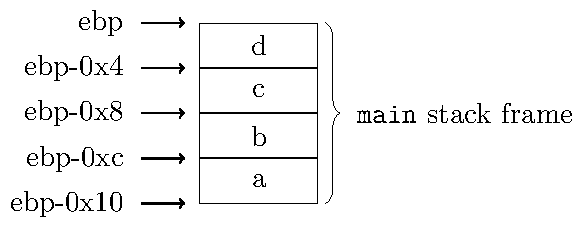
\includegraphics[page=1]{assembly/stack.pdf}
    \caption{Hàm \texttt{main}}
    \label{stack:1}
\end{figure}

Hình \ref{stack:1} có thể được giải thích khi dùng objdump ra đoạn assembly dưới đây.

\begin{lstlisting}[language={[x86masm]Assembler}]
000011c0 <main>:
    push   ebp
    mov    ebp,esp
    sub    esp,0x10
    call   1201 <__x86.get_pc_thunk.ax>
    add    eax,0x2e11
    mov    DWORD PTR [ebp-0x10],0x4
    mov    DWORD PTR [ebp-0xc],0x8
    push   DWORD PTR [ebp-0x10]
    call   118d <square>
    add    esp,0x4
    mov    DWORD PTR [ebp-0x8],eax
    push   DWORD PTR [ebp-0xc]
    call   11a2 <cube>
    add    esp,0x4
    mov    DWORD PTR [ebp-0x4],eax
    mov    eax,0x0
    leave  
    ret 
\end{lstlisting}

Biến \texttt{a} nằm ở vị trí 0x10 và biến \texttt{b} nằm ở vị trí 0xc. Vậy thì \texttt{a} nằm thấp hơn \texttt{b}. Điều này nghĩa là stack đi từ trên xuống.

Sau đó, giá trị 4 được chép qua biến \texttt{a}, giá trị 8 được chép qua biến \texttt{b}. Kế tiếp, trong hàm \texttt{main} gọi hàm \texttt{square}. Khi đó các tham số cần thiết cho hàm \texttt{square} sẽ được nạp vào stack (ở đây là biến \texttt{a} ở ebp-0x10) và hàm \texttt{square} sẽ được nạp vào stack \ref{stack:2}.

\begin{figure}[ht]
    \centering
    \includegraphics[page=2]{assembly/stack.pdf}
    \caption{Gọi hàm \texttt{square}}
    \label{stack:2}
\end{figure}

\underline{Bước 3. Gọi hàm \texttt{square}}. Hàm \texttt{square} có một tham số truyền vào là \texttt{a} ở địa chỉ ebp+0x8 (ebp mới của hàm \texttt{square}, không phải của \texttt{main}).

Ở đây, chương trình đưa giá trị 4 (ở ebp+0x8) vào thanh ghi eax và bình phương (lệnh \texttt{imult}). Kết quả trả về của hàm được gán trong thanh ghi eax.

\begin{lstlisting}[language={[x86masm]Assembler}]
0000118d <square>:
    push   ebp
    mov    ebp,esp
    call   1201 <__x86.get_pc_thunk.ax>
    add    eax,0x2e47
    mov    eax,DWORD PTR [ebp+0x8]
    imul   eax,eax
    pop    ebp
    ret 
\end{lstlisting}

%Kế tiếp, hàm \texttt{square} tính tích \texttt{local\_a * local\_a = 16} và lưu kết quả vừa tính vào lại \texttt{local\_a}. Sau đó hàm trả về giá trị của \texttt{local\_a} và lấy tất cả biến của hàm \texttt{square} trong stack ra.

%\includegraphics[scale=1]{stackheap/c2.PNG}

Sau khi hàm \texttt{square} chạy xong, nó gán giá trị 16 vào biến \texttt{c} (từ thanh ghi eax vào địa chỉ ebp-0x8), lúc này trong stack trở lại như lúc chưa có hàm \texttt{square}.

\underline{Bước 4. Gọi hàm \texttt{cube}}. Khi hàm \texttt{main} gọi hàm \texttt{cube}, nó thực hiện giống như cho hàm \texttt{square} ở trên, tức là tạo stack frame cho \texttt{cube} (hình \ref{stack:3}).

\begin{figure}[ht]
    \centering
    \includegraphics[page=3]{assembly/stack.pdf}
    \caption{Hàm \texttt{main} gọi hàm \texttt{cube}}
    \label{stack:3}
\end{figure}

\begin{lstlisting}[language={[x86masm]Assembler}]
000011a2 <cube>:
    push   ebp
    mov    ebp,esp
    call   1201 <__x86.get_pc_thunk.ax>
    add    eax,0x2e32
    push   DWORD PTR [ebp+0x8]
    call   118d <square>
    add    esp,0x4
    imul   eax,DWORD PTR [ebp+0x8]
    leave  
    ret
\end{lstlisting}

Tiếp theo, bên trong hàm \texttt{cube} lại gọi hàm \texttt{square} nên hàm \texttt{cube} sau khi đẩy các tham số cho hàm \texttt{square} vào stack thì gọi hàm \texttt{square} (hình \ref{stack:4}).

Sau khi hàm \texttt{square} thực hiện tính toán, giá trị trả về của nó được lưu trong eax. Sau đó hàm \texttt{cube} lấy kết quả ở eax (giá trị trả về của \texttt{square}) nhân với ebp+0x8 (tham số, ở đây là 8). Kết quả cuối cùng vẫn được lưu trữ ở eax để hàm \texttt{main} sử dụng.

\begin{figure}[ht]
    \centering
    \includegraphics[page=4]{assembly/stack.pdf}
    \caption{Hàm \texttt{cube} gọi hàm \texttt{square}}
    \label{stack:4}
\end{figure}

%\includegraphics[scale=1]{stackheap/c6.PNG}

%\includegraphics[scale=1]{stackheap/c4.PNG}

Cứ mỗi lần gọi hàm, hàm được gọi sẽ được nạp vào stack, và khi số lượng hàm quá lớn (có thể do đệ quy quá nhiều) sẽ gây tràn stack và gây ra lỗi stack overflow (tràn stack).

Do tất cả biến cục bộ được lưu trữ trong stack, nên trong mỗi hàm chỉ có thể có một số lượng biến nhất định. Vì vậy độ dài mảng cấp phát được thường là khá ít. Từ đó, một loại vùng nhớ được sử dụng để khắc phục nhược điểm này là heap.

\part{Quantum cryptography}

\parttoc

\chapter{Quantum computing}

\section{Qubit và toán tử quantum}

Trên máy tính hiện nay, đơn vị xử lý cơ bản là bit (0 hoặc 1). Trong máy tính lượng tử, đơn vị tính toán là qubit (quantum bit).

\subsection*{Qubit}

Mỗi qubit $\lvert \psi \rangle$ được biểu diễn dưới dạng tổ hợp tuyến tính của cơ sở gồm $\lvert 0 \rangle = (1, 0)$ và $\lvert 1 \rangle = (0, 1)$. Khi đó qubit $\lvert \psi \rangle = \alpha \lvert 0 \rangle + \beta \lvert 1 \rangle$. Ở đây $\alpha, \beta \in \mathbb{C}$ (tập số phức).

Tích của $n$ qubit là các tổ hợp $\lvert 0, 0, \ldots, 0 \rangle$, $\lvert 0, 0, \ldots, 1 \rangle$, ..., $\lvert 1, 1, \ldots, 1 \rangle$. Ta cũng ký hiệu $\lvert 0 \rangle \otimes \lvert 1 \rangle = \lvert 01 \rangle$. 

\begin{example}
    Nếu $\lvert \psi \rangle = \alpha \lvert 0 \rangle + \beta \lvert 1 \rangle$ và $\lvert \Psi \rangle = \gamma \lvert 0 \rangle + \delta \lvert 1 \rangle$ thì
    \begin{equation*}
        \lvert \psi \rangle \otimes \lvert \Psi \rangle = (\alpha \lvert 0 \rangle + \beta \lvert 1 \rangle) \otimes (\gamma \lvert 0 \rangle + \delta \lvert 1 \rangle) = \alpha \gamma \lvert 00 \rangle + \alpha \delta \lvert 0 1 \rangle + \beta \gamma \lvert 10 \rangle + \beta \delta \lvert 11 \rangle
    \end{equation*}
\end{example}

Tiếp theo là \textbf{toán tử quantum} và tương ứng với nó là các cổng (gate) trên mạch.

Toán tử quantum tác động lên một qubit hoặc tích của nhiều qubit.

Qubit có dạng $\lvert \psi \rangle = a \lvert 0 \rangle + b \lvert 1 \rangle$. Ta có thể viết hệ số dưới dạng vector cột $\begin{pmatrix} a \\ b \end{pmatrix}$. Khi đó, toán tử quantum sẽ là một ma trận $2 \times 2$ biến đổi vector trên thành vector mới $\begin{pmatrix} c \\ d \end{pmatrix}$ tương ứng với qubit $\lvert \Psi \rangle = c \lvert 0 \rangle + d \lvert 1 \rangle$.

Nói cách khác, đặt toán tử quantum là ma trận $\mathcal{U} = \begin{pmatrix} c_{11} & c_{12} \\ c_{21} & c_{22} \end{pmatrix}$ thì ta có
\begin{equation*}
    \lvert \psi \rangle \to \lvert \Psi \rangle = \mathcal{U} \lvert \psi \rangle, \quad \begin{pmatrix} c_{11} & c_{12} \\ c_{21} & c_{22} \end{pmatrix} \cdot \begin{pmatrix} a \\ b \end{pmatrix} = \begin{pmatrix} c \\ d \end{pmatrix}
\end{equation*}

\subsection*{Các toán tử quantum thường gặp}

\begin{definition}[Toán tử đồng nhất]
    Toán tử đồng nhất identity giữ nguyên qubit đầu vào. Ma trận tương ứng là ma trận đơn vị $I = \begin{pmatrix} 1 & 0 \\ 0 & 1 \end{pmatrix}$.
\end{definition}

\begin{definition}[Toán tử NOT]
    Toán tử NOT có ma trận tương ứng là $\text{NOT} = \begin{pmatrix} 0 & 1 \\ 1 & 0 \end{pmatrix}$. Khi đó $\text{NOT} \lvert \psi \rangle = b \lvert 0 \rangle + a \lvert 1 \rangle$ với $x \in \{ 0, 1 \}$.
\end{definition}

Khi qubit là $\lvert 0 \rangle$ hoặc $\lvert 1 \rangle$, tác dụng của toán tử NOT là phép XOR nên ta có $\text{NOT} \lvert x \rangle = \lvert x \oplus 1 \rangle$.

\begin{definition}[Toán tử Hadamard]
    Ma trận của toán tử Hadamard là $H = \dfrac{1}{\sqrt{2}} \begin{pmatrix} 1 & 1 \\ 1 & - 1 \end{pmatrix}$. 
\end{definition}

\begin{example}
    Xét qubit $\lvert \psi \rangle = a \lvert 0 \rangle + b \lvert 1 \rangle$, toán tử Hadamard tương ứng với phép nhân ma trận
    \begin{equation*}
        \dfrac{1}{\sqrt{2}} \begin{pmatrix} 1 & 1 \\ 1 & - 1 \end{pmatrix} \cdot \begin{pmatrix} a \\ b \end{pmatrix} = \begin{pmatrix} \dfrac{1}{\sqrt{2}} (a + b) \\ \dfrac{1}{\sqrt{2}} (a - b) \end{pmatrix}
    \end{equation*}

    Ta chuyển cột kết quả về lại dạng tổ hợp tuyến tính thì cổng Hadamard hoạt động trên qubit $\lvert \psi \rangle = a \lvert 0 \rangle + b \lvert 1 \rangle$ cho kết quả là
    \begin{equation*}
        H \lvert \psi \rangle = H(a \lvert 0 \rangle + b \lvert 1 \rangle) = \dfrac{1}{\sqrt{2}} (a + b) \lvert 0 \rangle + \dfrac{1}{\sqrt{2}} (a - b) \lvert 1 \rangle
    \end{equation*}
\end{example}

Nếu $\lvert \psi \rangle \equiv \lvert 0 \rangle$ thì tương đương với $a = 1, b = 0$. Ta có $H \lvert 0 \rangle = \dfrac{\lvert 0 \rangle + \lvert 1 \rangle}{\sqrt{2}}$.

Nếu $\lvert \psi \rangle \equiv \lvert 1 \rangle$ thì tương đương với $a = 0, b = 1$. Ta có $H \lvert 1 \rangle = \dfrac{\lvert 0 \rangle - \lvert 1 \rangle}{\sqrt{2}}$.

Tổng quát ta nhận thấy, với $x \in \{ 0, 1 \}$ thì $H \lvert x \rangle = \dfrac{\lvert 0 \rangle + (-1)^x \lvert 1 \rangle}{\sqrt{2}}$.

Ta thấy rằng toán tử ngược của toán tử Hadamard là chính nó.

Tiếp theo là toán tử thường được dùng nhất khi tính toán trên tích của nhiều qubit: toán tử control.

Như đã xem xét ở trên, tích của $n$ qubit sẽ có $2^n$ phần tử tương ứng các bộ $\lvert 0, 0, \ldots, 0, 0 \rangle$, $\lvert 0, 0, \ldots, 0, 1 \rangle$, ... Do đó toán tử control sẽ là ma trận kích thước $2^n \times 2^n$.


\begin{definition}[Toán tử control]    
    Gọi $\mathcal{U} = \begin{pmatrix} c_{11} & c_{12} \\ c_{21} & c_{22} \end{pmatrix}$ là toán tử tác động lên một qubit (ví dụ như 3 toán tử đã đề cập). Xét hai qubit là $\lvert x \rangle = a \lvert 0 \rangle + b \lvert 1 \rangle$ và $\lvert y \rangle = c \lvert 0 \rangle + d \lvert 1 \rangle$. Từ phía trên
    \begin{equation*}
        \lvert x \rangle \otimes \lvert y \rangle = ac \lvert 00 \rangle + ad \lvert 01 \rangle + bc \lvert 10 \rangle + bd \lvert 11 \rangle
    \end{equation*}

    Khi đó toán tử control có dạng ma trận là
    \begin{equation*}
        c \mathcal{U} = \begin{pmatrix} 1 & 0 & 0 & 0 \\ 0 & 1 & 0 & 0 \\ 0 & 0 & c_{11} & c_{12} \\ 0 & 0 & c_{21} & c_{22} \end{pmatrix}
    \end{equation*}

    Hay viết dưới dạng ma trận khối là $c \mathcal{U} = \begin{pmatrix} I & \mathcal{O} \\ \mathcal{O} & \mathcal{U} \end{pmatrix}$.
\end{definition}

Ta cũng viết tích $\lvert x \rangle \otimes \lvert y \rangle$ dưới dạng vector cột (4 phần tử). Khi đó
\begin{equation*}
    \mathcal{U} (\lvert x \rangle \otimes \lvert y \rangle) = \begin{pmatrix} 1 & 0 & 0 & 0 \\ 0 & 1 & 0 & 0 \\ 0 & 0 & c_{11} & c_{12} \\ 0 & 0 & c_{21} & c_{22} \end{pmatrix} \cdot \begin{pmatrix} ac \\ ad \\ bc \\ bd \end{pmatrix} = \begin{pmatrix} ac \\ ad \\ c_{11} \cdot bc + c_{12} \cdot bd \\ c_{21} \cdot bc + c_{22} \cdot bd \end{pmatrix}
\end{equation*}

Hai phần tử đầu của vector kết quả không thay đổi, còn phần sau có "một phần" là $\mathcal{U} \lvert y \rangle$. Khi viết lại kết quả dưới dạng qubit thì
\begin{equation*}
    ac \lvert 00 \rangle + ad \lvert 01 \rangle + (c_{11} \cdot bc + c_{12} \cdot bd) \lvert 10 \rangle + (c_{21} \cdot bc + c_{22} \cdot bd) \lvert 11 \rangle
\end{equation*}

Ta có một số nhận xét sau đây.

Nếu $\lvert x \rangle \equiv \lvert 0 \rangle$, tức là $a = 1, b = 0$ thì tích trên tương ứng với $c \lvert 00 \rangle + d \lvert 01 \rangle + 0 \lvert 10 \rangle + 0 \lvert 11 \rangle = \lvert 0 \rangle \otimes (c \lvert 0 \rangle + d \lvert 1 \rangle) = \lvert x \rangle \otimes \lvert y \rangle$.

Nếu $\lvert x \rangle \equiv \lvert 1 \rangle$, tức là $a = 0, b = 1$ thì tích trên tương ứng với $0 \lvert 00 \rangle + 0 \lvert 01 \rangle + (c_{11} c + c_{12} d) \lvert 10 \rangle + (c_{21} c + c_{22} d) \lvert 11 \rangle = \lvert 1 \rangle \otimes ((c_{11} c + c_{12} d) \lvert 0 \rangle + (c_{21} c + c_{22} d) \lvert 1 \rangle) = \lvert 1 \rangle \otimes \mathcal{U} \lvert y \rangle = \lvert x \rangle \otimes \mathcal{U} \lvert y \rangle$.

Tổng kết lại, với $x \in \{ 0, 1\}$ thì

\begin{itemize}
    \item nếu $x = 0$ thì $\lvert x \rangle \otimes \lvert y \rangle \to \lvert x \rangle \otimes \lvert y \rangle$.
    \item nếu $x = 1$ thì $\lvert x \rangle \otimes \lvert y \rangle \to \lvert x \rangle \otimes \mathcal{U} \lvert y \rangle$.
\end{itemize}

Tùy vào $x$ là 0 hay 1 mà toán tử quantum $\mathcal{U}$ sẽ bị bỏ qua hoặc xem xét. Ở đây qubit $\lvert x \rangle$ đóng vai trò điều khiển nên đây được gọi là toán tử control.

\begin{definition}[Toán tử control CNOT (Control NOT)]
    Toán tử quantum CNOT có ma trận là
    \begin{equation*}
        \begin{pmatrix} 1 & 0 & 0 & 0 \\ 0 & 1 & 0 & 0 \\ 0 & 0 & 0 & 1 \\ 0 & 0 & 1 & 0 \end{pmatrix} = \begin{pmatrix} I & \mathcal{O} \\ \mathcal{O} & \text{NOT} \end{pmatrix}
    \end{equation*}
\end{definition}

Qubit $\lvert x \rangle$ với $x \in \{ 0, 1 \}$ đóng vai trò control cho qubit $\lvert y \rangle$. Khi $x \equiv 0$ thì $y$ giữ nguyên, hay $\lvert y \oplus 0 \rangle = \lvert y \oplus x \rangle$. Khi $x \equiv 1$ thì áp dụng cổng NOT bên trên, khi đó $y$ biến đổi thành $y \oplus 1 = y \oplus x$.

\subimport{code_based_cryptography/}{code_crypto.tex}

\part{Post-quantum cryptography}

\parttoc

\subimport{lattice_based_cryptography/}{lattice_crypto.tex}

{
\hyphenpenalty=10000 \spaceskip=0.4em plus 0.8em minus 0.35em
\printbibliography[env=gostbibliography,heading=bibintoc,title={Tài liệu tham khảo}]
}

%\appendix

\part{Các cuộc thi và bài tập trong sách}

\parttoc

\subimport{nsucrypto}{nsucrypto.tex}

\subimport{olympiad/CryptoFox/}{cryptofox2024.tex}

\subimport{contests}{onthi.tex}

\part{Những điều nhỏ xíu}

\parttoc

\subimport{./}{partial_derivaties.tex}

\chapter{Đại số nâng cao}

\section{Đa thức nội suy Lagrange}

Trong đại số, công thức nội suy Lagrange cho phép chúng ta tìm được một đa thức $f(x)$ trên trường $\FF$ bất kì khi biết được một số cặp $(x_i, f(x_i))$ nhất định ($x_i, f(x_i) \in \FF$).

Để tìm đa thức $f(x)$ có bậc $n$ ta cần ít nhất $n+1$ cặp $(x_i, f(x_i) = y_i)$, với $1 \leqslant i \leqslant n+1$ và $x_i \neq x_j$ với mọi $i \neq j$.

Khi đó, ta có \textbf{công thức nội suy Lagrange} như sau:

\begin{equation*}
    \displaystyle{f(x) = \sum_{i=1}^{n+1} \left(y_i \cdot \prod_{j \neq i} \frac{x - x_j}{x_i - x_j}\right)}
\end{equation*}

\begin{example}
    Giả sử chúng ta có hàm $f(x) = x^2 + x + 1$. Khi đó $f(1) = 3, f(-1) = 1, f(0) = 1$.

    Từ ba cặp $(x_i, f(x_i))$ trên mình sẽ tìm ngược lại $f(x)$ ban đầu.

    Theo công thức thì
    \begin{align*}
        f(x) = & y_1 \cdot \frac{(x - x_2) (x - x_3)}{(x_1 - x_2) (x_1 - x_3)} + y_2 \cdot \frac{(x - x1) (x - x_3)}{(x_2 - x_1) (x_2 - x_3)} \\
        + & y_3 \cdot \frac{(x - x1) (x - x_2)}{(x_3 - x1) (x_3 - x_2)}
    \end{align*}
    Thay số vào thì ta có
    \begin{equation*}
        \displaystyle{f(x) = 3 \cdot \frac{(x - (-1)) (x - 0)}{(1 - (-1)) (1 - 0)} + 1 \cdot \frac{(x - 1) (x - 0)}{(-1 - 1) (-1 - 0)} + 1 \cdot \frac{(x - 1) (x - (-1))}{(0 - 1) (0 - (-1))}}
    \end{equation*}

    Thu gọn lại ta có $f(x) = x^2 + x + 1$ (đúng với hàm cần tìm).
\end{example}


\end{document}